\input{"preamble.tex"}

\addbibresource{FloerHomology.bib}

\let\Begin\begin
\let\End\end
\newcommand\wrapenv[1]{#1}

\makeatletter
\def\ScaleWidthIfNeeded{%
 \ifdim\Gin@nat@width>\linewidth
    \linewidth
  \else
    \Gin@nat@width
  \fi
}
\def\ScaleHeightIfNeeded{%
  \ifdim\Gin@nat@height>0.9\textheight
    0.9\textheight
  \else
    \Gin@nat@width
  \fi
}
\makeatother

\setkeys{Gin}{width=\ScaleWidthIfNeeded,height=\ScaleHeightIfNeeded,keepaspectratio}%

\title{
\rule{\linewidth}{1pt} \\
\textbf{
    Floer Homology
  }
    \\ {\normalsize Lectures by Akram Alishahi. University of Georgia,
Spring 2021} \\
  \rule{\linewidth}{2pt}
}
\titlehead{
    \begin{center}
  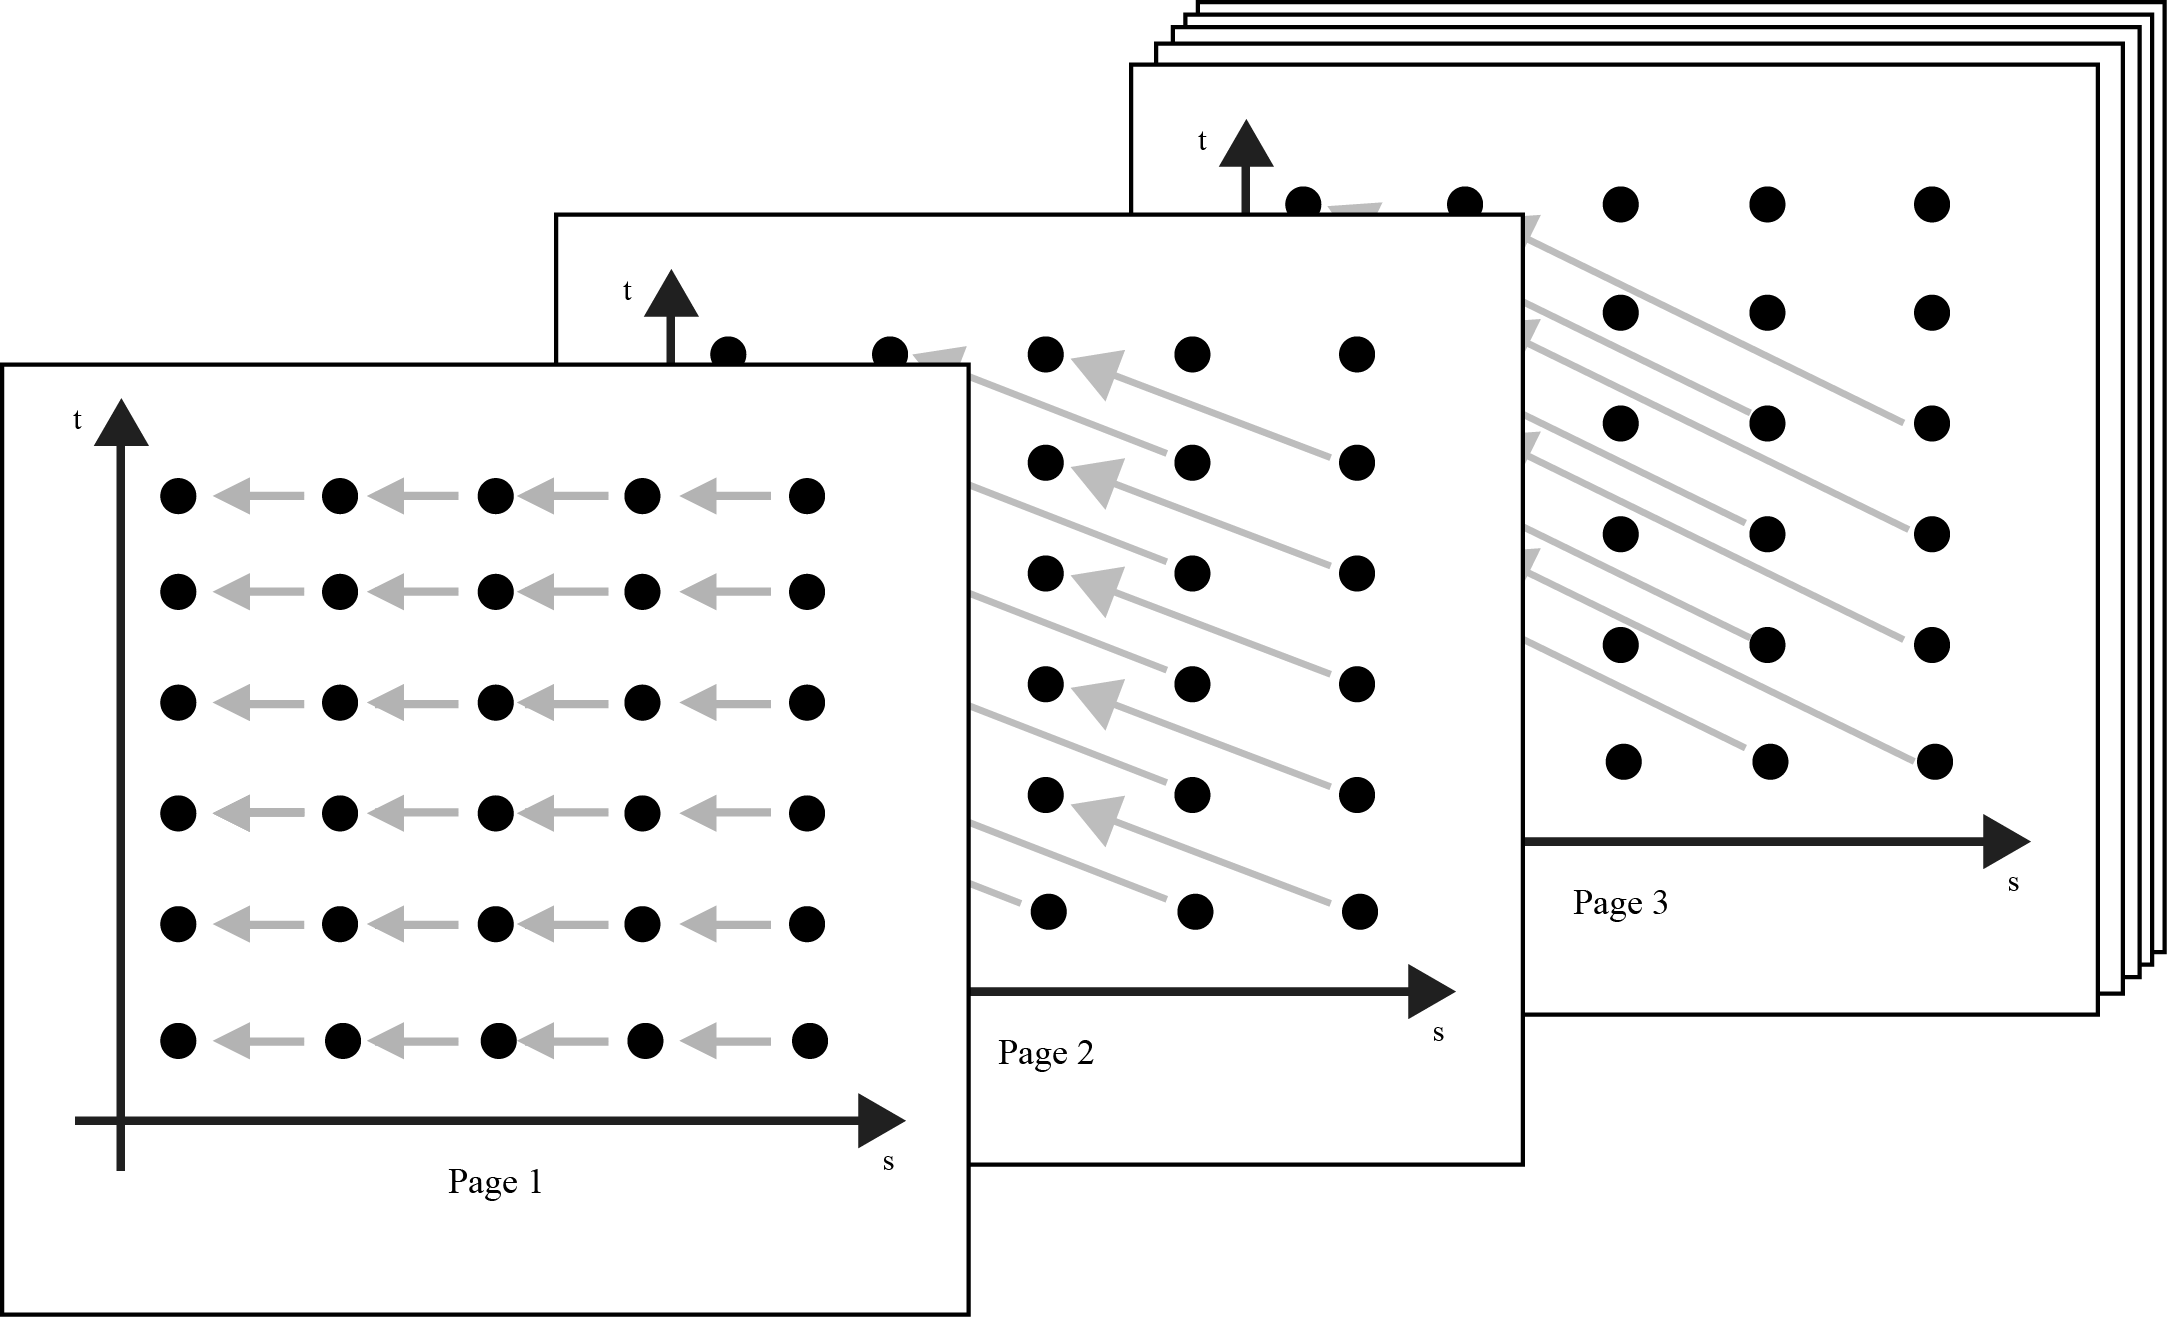
\includegraphics[width=\linewidth,height=0.45\textheight,keepaspectratio]{figures/cover.png}
  \end{center}
       \begin{minipage}{.35\linewidth}
    \begin{flushleft}
      \vspace{2em}
      {\fontsize{6pt}{2pt} \textit{Notes: These are notes live-tex'd
from a graduate course in Floer Homology taught by Akram Alishahi at the
University of Georgia in Spring 2021. As such, any errors or
inaccuracies are almost certainly my own. } } \\
    \end{flushleft}
    \end{minipage}
    \hfill
    \begin{minipage}{.65\linewidth}
    \end{minipage}
  }







\begin{document}

\date{}
\author{D. Zack Garza}
\maketitle
\begin{flushleft}
\textit{D. Zack Garza} \\
\textit{University of Georgia} \\
  \textit{\href{mailto: dzackgarza@gmail.com}{dzackgarza@gmail.com}} \\
{\tiny \textit{Last updated:} 2021-01-28 }
\end{flushleft}


\newpage

% Note: addsec only in KomaScript
\addsec{Table of Contents}
\tableofcontents
\newpage

\def\contradiction
{
\tikz[baseline, x=0.2em, y=0.2em, line width=0.04em]
\draw (0,0) -- ({4*cos(45)},{4*sin(45)})
    (-1,1) -- ({-1 + 4*cos(45)},{1 + 4*sin(45)})
    (-1,3) -- ({-1 + 4*cos(315)},{3 + 4*sin(315)})
    (0,4) -- ({0 + 4*cos(315)},{4 + 4*sin(315)});
}

\hypertarget{lecture-1-overview-wednesday-january-13}{%
\section{Lecture 1: Overview (Wednesday, January
13)}\label{lecture-1-overview-wednesday-january-13}}

\hypertarget{course-logistics}{%
\subsection{Course Logistics}\label{course-logistics}}

\begin{quote}
Note (DZG): Everything in this section comes from Akram!
\end{quote}

\hypertarget{description}{%
\subsubsection{Description}\label{description}}

``I am teaching a topics course about Heegaard Floer homology next
semester. Heegaard Floer homology was defined by Peter Ozsváth and
Zoltan Szabó around 2000. It is a package of powerful invariants of
smooth 3- and 4-manifolds, knots/links and contact structures. Over the
last two decades, it has become a central tool in low-dimensional
topology. It has been used extensively to study and resolve important
questions concerning unknotting number, slice genus, knot concordance
and Dehn surgery. It has been employed in critical ways to study taut
foliations, contact structures and smooth 4-manifolds. There are also
many rich connections between Heegaard Floer homology and other manifold
and knot invariants coming from gauge theory as well as representation
theory. We will learn the basic construction of Heegaard Floer homology,
starting with the definition of the 3-manifold and knot invariants. In
the second half of this course, we will turn to computations and
applications of the theory to low-dimensional topology and knot theory.
In particular, several numerical invariants have been defined using this
homological invariants. At the end of the semester, I would expect each
one of you to learn the construction of one of these invariants (of
course with my help) and present it to the class.''

\hypertarget{expository-papers}{%
\subsubsection{Expository Papers}\label{expository-papers}}

\begin{itemize}
\tightlist
\item
  \autocite{G} J. Greene,
  \href{https://www.ams.org/journals/notices/202101/rnoti-p19.pdf}{Heegaard
  Floer homology}
\item
  \autocite{H} J. Hom,
  \href{https://arxiv.org/pdf/2008.01836.pdf}{Lecture notes on Heegaard
  Floer homology}
\item
  \autocite{L} R. Lipshitz,
  \href{https://arxiv.org/abs/1411.4540}{Heegaard Floer homologies}
\item
  \autocite{M} C. Manolescu, \href{https://arxiv.org/abs/1401.7107}{An
  introduction to knot Floer homology}
\item
  \autocite{OS-1} P. Ozsváth and Z. Szabó,
  \href{https://web.math.princeton.edu/~petero/Introduction.pdf}{An
  introduction to Heegaard Floer homology}
\item
  \autocite{OS-2} P. Ozsváth and Z. Szabó,
  \href{https://web.math.princeton.edu/~petero/Lectures.pdf}{Lectures on
  Heegaard Floer homology}
\item
  \autocite{OS-3} P. Ozsváth and Z. Szabó,
  \href{https://arxiv.org/pdf/math/0403029.pdf}{Heegaard diagrams and
  holomorphic disks}
\end{itemize}

\hypertarget{research-papers}{%
\subsubsection{Research Papers}\label{research-papers}}

\begin{itemize}
\tightlist
\item
  \autocite{OSz04a} Peter Ozsváth and Zoltán Szabó, Holomorphic disks
  and topological invariants for closed three-manifolds. Ann. of Math.
  (2) 159 (2004), no. 3, 1027--1158.
  \href{https://arxiv.org/abs/math/0101206}{arXiv:math/0101206}
\item
  \autocite{OSz04b} Peter Ozsváth and Zoltán Szabó, Holomorphic disks
  and three-manifold invariants: properties and applications. Ann. of
  Math. (2) 159 (2004), no. 3, 1159--1245.
  \href{https://arxiv.org/abs/math/0105202}{arXiv:math/0105202}
\item
  \autocite{OSz04c} Peter Ozsváth and Zoltán Szabó, Holomorphic disks
  and knot invariants. Adv. Math. 186 (2004), no. 1, 58--116.
  \href{https://arxiv.org/abs/math/0209056}{arXiv:math/0209056}
\item
  \autocite{OSz06} Peter Ozsváth and Zoltán Szabó, Holomorphic triangles
  and invariants for smooth four manifolds. Adv. Math. 202 (2006), no.
  2, 326--400.
  \href{https://arxiv.org/abs/math/0110169}{arXiv:math/0110169}
\item
  \autocite{Per08} Timothy Perutz, Hamiltonian handleslides for Heegaard
  Floer homology. Proceedings of Gökova Geometry-Topology Conference
  2007, 15--35, Gökova Geometry/Topology Conference (GGT), Gökova, 2008.
  \href{https://arxiv.org/abs/0801.0564}{arXiv:0801.0564}
\end{itemize}

\hypertarget{basic-morse-theory-symplectic-geometry-and-floer-homology}{%
\subsubsection{Basic Morse Theory, Symplectic Geometry and Floer
Homology}\label{basic-morse-theory-symplectic-geometry-and-floer-homology}}

\begin{itemize}
\tightlist
\item
  \autocite{Mi-1} Milnor,
  \href{https://press.princeton.edu/books/paperback/9780691080086/morse-theory-am-51-volume-51}{Morse
  theory}
\item
  \autocite{Mi-2} Milnor,
  \href{https://press.princeton.edu/books/hardcover/9780691651132/lectures-on-the-h-cobordism-theorem}{Lectures
  on the \(h{\hbox{-}}\)cobordism theorem}
\item
  \autocite{Ca} A. Cannas da Silva.
  \href{https://www.springer.com/gp/book/9783540421955}{Lectures on
  Symplectic Geometry}
\item
  \autocite{Mc} D. McDuff,
  \href{http://www.math.stonybrook.edu/~dusa/floer8.pdf}{Floer theory
  and low-dimensional topology}
\item
  \autocite{AD} M. Audin and M. Damian,
  \href{https://link.springer.com/book/10.1007/978-1-4471-5496-9}{Morse
  theory and Floer homology}
\item
  \autocite{Hu} M. Hutchings,
  \href{https://math.berkeley.edu/~hutching/teach/276-2010/mfp.ps}{Lecture
  notes on Morse homology (with an eye towards Floer theory and
  pseudoholomorphic curves)}
\end{itemize}

\hypertarget{low-dimensional-topology}{%
\subsubsection{Low-dimensional
Topology}\label{low-dimensional-topology}}

\begin{itemize}
\tightlist
\item
  \autocite{S} N. Saveliev,
  \href{https://www.degruyter.com/view/title/121170}{Lectures on the
  topology of 3-manifolds}
\item
  \autocite{R} D. Rolfsen,
  \href{https://bookstore.ams.org/chel-346-h/}{Knots and links}
\item
  \autocite{GS} R. Gompf and A. Stipsicz,
  \href{https://bookstore.ams.org/gsm-20}{4-manifolds and Kirby
  calculus}
\item
  \autocite{L} R. Lickorish,
  \href{https://link.springer.com/book/10.1007/978-1-4612-0691-0}{An
  introduction to knot theory}
\end{itemize}

\hypertarget{suggested-topics-for-presentations}{%
\subsubsection{Suggested Topics for
Presentations}\label{suggested-topics-for-presentations}}

\begin{itemize}
\item
  \autocite{SW} S. Sarkar and J. Wang, {[}An algorithm for computing
  some Heegaard Floer homologies, Ann. of Math., 171 (2010), 1213--1236,
  \href{https://arxiv.org/abs/math/0607777}{arXiv:math/0607777}.
\item
  Grid homology from:

  \begin{itemize}
  \item
    C. Manolescu and P. Ozsváth and S. Sarkar,
    \href{https://annals.math.princeton.edu/wp-content/uploads/annals-v169-n2-p07.pdf}{A
    combinatorial description of knot Floer homology}, Ann. of Math.,
    169 (2009), 633--660,
    \href{https://arxiv.org/abs/math/0607691}{arXiv:math/0607691}.
  \item
    P. Ozsváth and A. Stipsicz and Z. Szabó,
    \href{https://bookstore.ams.org/surv-208}{Grid Homology for Knots
    and Links},

    \begin{itemize}
    \tightlist
    \item
      Also available
      \href{https://web.math.princeton.edu/~petero/GridHomologyBook.pdf}{here}
      with comment: please go and buy a hard copy, too!
    \end{itemize}
  \end{itemize}
\item
  J. Hom,
  \href{https://www.worldscientific.com/doi/abs/10.1142/S0218216517400156}{A
  survey on Heegaard Floer homology and concordance} J. of Knot Theo.
  and Its Ram.(2) 26 (2017)
  \href{https://arxiv.org/abs/1512.00383}{arXiv:1512.00383}
\item
  K. Honda and W. Kazez and G. Matić,
  \href{https://projecteuclid.org/euclid.jdg/1261495333}{On the contact
  class in Heegaard Floer homology}, J. Differential Geom. (2) 83
  (2009), 289-311,
  \href{https://arxiv.org/abs/math/0609734}{arXiv:math/0609734}
\item
  Sutured Floer homology from:

  \begin{itemize}
  \tightlist
  \item
    \autocite{L} Lipshitz expository paper listed above
  \item
    A. Juhász
    \href{https://projecteuclid.org/euclid.agt/1513796585}{Holomorphic
    discs and sutured manifolds} Algebr. Geom. Topol., (3) 6 (2006),
    1429-1457,
    \href{https://arxiv.org/abs/math/0601443}{arXiv:math/0601443}
  \item
    A. Juhász,
    \href{https://projecteuclid.org/euclid.agt/1513796824}{Knot Floer
    homology and Seifert surfaces} Algebr. Geom. Topol., (1) 8 (2008),
    603-608
    \href{https://arxiv.org/abs/math/0702514}{arxiv:math/0702514}
  \end{itemize}
\end{itemize}

\todo[inline]{Convert to bibtex?}

\hypertarget{intro-and-motivation}{%
\subsection{Intro and Motivation}\label{intro-and-motivation}}

We'll assume everything is smooth and oriented.

\begin{proposition}[Osvath-Szabo (2000)]

To closed 3-manifolds \(M\) we can assign a graded abelian group
\(\widehat{HF}(M)\), which can be computed combinatorially \footnote{See
  Sarkour-Wang} . There are several variants:

\begin{itemize}
\item
  \(HF^- \in {\operatorname{grMod}}({\mathbb{Z}}_2[u])\), \footnote{This
    is the strongest variant.}
\item
  \(HF^+ \in {\operatorname{Mod}}({\mathbb{Z}}_2[u, u ^{-1} ] / u {\mathbb{Z}}_2[u])\).
\item
  \(HF^\infty \in {\operatorname{grMod}}({\mathbb{Z}}_2[u, u ^{-1} ])\),
\end{itemize}

\(HF^+\) and \(HF^\infty\) can be computed using \(HF^-\). In general,
we'll write \(HF^{\,\cdot\,}\) to denote constructions that work with
any of the above variants.

\end{proposition}

\begin{remark}

Note that \({\mathbb{Z}}_2\) can be replaced with \({\mathbb{Z}}\), but
it's technical and we won't discuss it here. For the first half of the
course, we'll just discuss \(\widehat{HF}\), and we'll discuss the
latter 3 in the second half.

\end{remark}

\hypertarget{geometric-information}{%
\subsubsection{Geometric Information}\label{geometric-information}}

These invariants can be used to compute the \textbf{Thurston seminorm}
of a 3-manifold:

\begin{definition}[Thurston Seminorm]

A homology class \(\alpha\in H_2(M)\) can be represented as
\(\alpha\in [S]\) for \(S\) a closed surface whose fundamental class
represents \(\alpha\) where \(S = \bigcup_{i=1}^n S_i\) can be a union
of closed embedded surfaces \(S_i\). Then we first compute
\begin{align*}
\max\left\{{0, - \chi(S_i) }\right\} 
=
\begin{cases}
0 & \text{if } S_i \cong {\mathbb{S}}^2, {\mathbb{T}}^2 \\ 
\\
- \chi(S_i) = 2g(S_i) - 2  & \text{ else} .
\end{cases}
.\end{align*}
Note that the max checks if \(\chi\) is positive. Then define
\begin{align*}
{\left\lVert { \alpha } \right\rVert} \coloneqq\min_S \qty{ \sum_{i=1}^n 
\max\left\{{0, - \chi(S_i) }\right\} }
,\end{align*}
where we sum over the embedded subsurfaces and check which overall
surface gives the smallest norm.

\end{definition}

\begin{remark}

Note that this can't be a norm, since if
\({\mathbb{S}}^2, {\mathbb{T}}^2 \in [S] \implies {\left\lVert {\alpha } \right\rVert}= 0\).

\end{remark}

\begin{theorem}[Osvath-Szabo]

\(HF\) detects \footnote{What does ``detect'' mean? This is slightly
  technical.} the Thurston seminorm, and there is a splitting as
groups/modules
\begin{align*}
HF^{\,\cdot\,}(M) = \bigoplus _{\mathfrak{s} \in {\operatorname{Spin}}^c(M)} HF^{\,\cdot\,}(M, S) 
\end{align*}
where \(S \in {\operatorname{Spin}}^c(M)\) is a \textbf{spin\(^c\)
structure}: an oriented 2-dimensional vector bundle on \(M\) (up to some
equivalence).

\end{theorem}

\begin{remark}

The Thurston norm \({\left\lVert {a} \right\rVert}\) can be computed
from this data by considering a perturbed version of \(\widehat{HF}\),
denoted \(\underline{\widehat{HF}}\), in the following way: taking the
first Chern class \(c_1(\mathfrak{s}) \in H^2(M)\) (which can be
associated to every 2-dimensional vector bundle), we have
\begin{align*}
{\left\lVert { \alpha} \right\rVert} = \max_{\underline{\widehat{HF}}(M, \mathfrak{s}  ) \neq 0 }
{\left\lvert {{\left\langle { c_1(\mathfrak{s})  },~{ \alpha } \right\rangle}  } \right\rvert}
.\end{align*}

\end{remark}

\begin{slogan}

Floer homology groups split over these spin\(^c\) structures and can be
used to compute Thurston norms.

\end{slogan}

\begin{theorem}[Ni]

Given \(F \subseteq M\) with genus \(g\geq 2\), \(HF\) detects if \(M\)
\emph{fibers} over \(S^1\) with \(F\) as a fiber, i.e.~there exists a
fiber bundle

\begin{center}
\begin{tikzcd}
F 
  \ar[r, hook] 
& 
M
  \ar[d, "\pi"] 
\\
& 
S^1 
\end{tikzcd}
\end{center}

This uses the existence of the splitting over spin\(^c\) structures and
uses \(HF^+\) in the following way: such a bundles exists if and only if
\begin{align*}
\bigoplus _{{\left\langle { c_1(\mathfrak{s}) },~{ [F] } \right\rangle}  =2g-2} HF^+(M, \mathfrak{s}) = {\mathbb{Z}}
.\end{align*}

\end{theorem}

\begin{definition}[Contact Structure]

Equivalently,

\begin{itemize}
\item
  A smooth oriented nowhere integrable 2-plane field \(\xi\), or
\item
  A 2-plane field \(\xi \coloneqq\ker( \alpha)\) where \(\alpha\) is a
  1-form such that \(\alpha\wedge d \alpha > 0\). \footnote{Note that
    wedging to a nontrivial top form is equivalent to being nowhere
    integrable here.}
\end{itemize}

\end{definition}

\begin{example}[?]

The standard contact structure on \({\mathbb{R}}^3\) is given by
\begin{align*}
\alpha\coloneqq dz - ydz
,\end{align*}
which yields the following 2-plane field \(\xi \coloneqq\ker \alpha\):

\begin{figure}
\centering
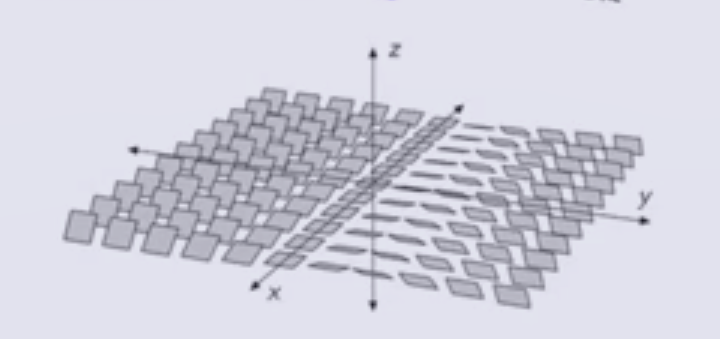
\includegraphics{figures/image_2021-01-18-23-04-19.png}
\caption{2-Plane Field in \({\mathbb{R}}^3\)}
\end{figure}

You can see that \(z=0 \implies y=0\), so the \(xy{\hbox{-}}\)plane is
in the kernel, yielding the flat planes down the middle:

\begin{figure}
\centering
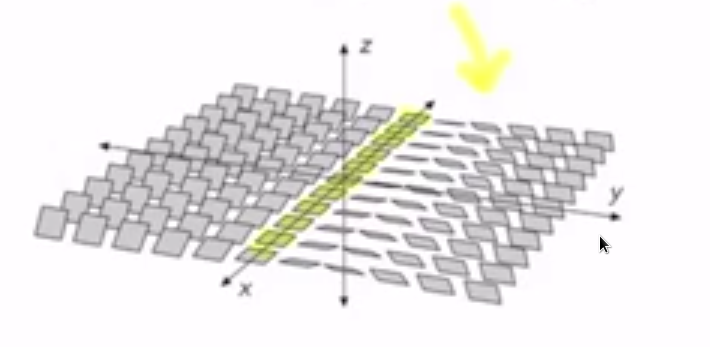
\includegraphics{figures/Flat_Planes.png}
\caption{Flat Planes}
\end{figure}

\end{example}

\begin{proposition}[Contact Class (Osvath-Szabo-Honda-Kazez-Matic)]

To each such \(\xi\) one can associate a \textbf{contact class}
\(c(\xi) \in \widehat{HF}(-M)\), where \(-M\) is \(M\) with the reversed
orientation.

\end{proposition}

\begin{remark}

This gives obstructions for two of the following important properties of
contact structures:

\begin{itemize}
\tightlist
\item
  Being \textbf{overtwisted}, or
\item
  Being \textbf{Stein fillable}.
\end{itemize}

\end{remark}

\begin{theorem}[?]

\envlist

\begin{itemize}
\tightlist
\item
  If \(\xi\) is overtwisted, then \(c(\xi) = 0\).
\item
  If \(\xi\) is Stein fillable, then \(c(\xi) \neq 0\).
\end{itemize}

\end{theorem}

We'll also discuss similar invariants for knots that were created after
these invariants for manifolds.

\begin{definition}[Knots]

Recall that a \textbf{knot} is an embedding \(S^1 \hookrightarrow M\).

\begin{figure}
\centering
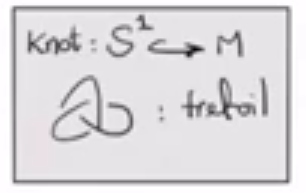
\includegraphics[width=1.5625in,height=\textheight]{figures/image_2021-01-18-23-13-07.png}
\caption{Example: the trefoil knot}
\end{figure}

\end{definition}

\begin{proposition}[Knot Floer Homology (Ozsváth-Szabó)]

Given a knot \(K \subseteq M\) a 3-manifold (e.g.~\(M = S^3\)), there is
extra algebraic structure on \(\widehat{CF}(M)\): a filtration. These
allow defining a new bigraded abelian group \(\widehat{HFK}(M, K)\)
(which is also a \({\mathbb{Z}}_2{\hbox{-}}\)vector space) that takes
includes the information of \(K\). This yields a decomposition
\begin{align*}
\widehat{HFK}(M, K) = \bigoplus _{m, a} \widehat{HFK}_m(M, K, a)
.\end{align*}

This similarly works for other variants: there is a filtration on
\(CF^-(M)\) which yields \(HFK^-(M, K)\), a bigraded
\({\mathbb{Z}}_2[u]{\hbox{-}}\)module.

\end{proposition}

Some properties of Knot Floer Homology:

\begin{fact}

\(\widehat{HFK}(K)\) categorifies the Alexander polynomial
\(\Delta_K(t)\) of \(K\), i.e.~taking the graded Euler characteristic
yields
\begin{align*}
\Delta_K (t) =\sum_{m, a} (-1)^m\qty{ \dim \widehat{HFK}_m(K, a) } t^a
.\end{align*}

\end{fact}

\begin{fact}

\(\widehat{HFK}(K)\) detects the \textbf{Seifert genus} of a knot
\(g(K)\), defined as the smallest \(g\) such that there exists an
embedded surface \footnote{These are referred to as \textbf{Seifert
  surfaces}.} \(F\) of genus \(g\) in \(S^3\) that bounds \(K\), so
\({{\partial}}F = K\).

\begin{example}[The Unknot]

The unknot bounds a disc, so its genus is zero:

\begin{figure}
\centering
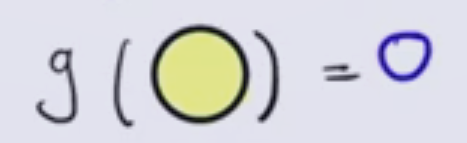
\includegraphics{figures/image_2021-01-18-23-29-23.png}
\caption{The genus of the unknot}
\end{figure}

\end{example}

\begin{exercise}[The Trefoil]

Using the ``outside'' disc on the trefoil, find 3 bands that show its
genus is 1.

\begin{figure}
\centering
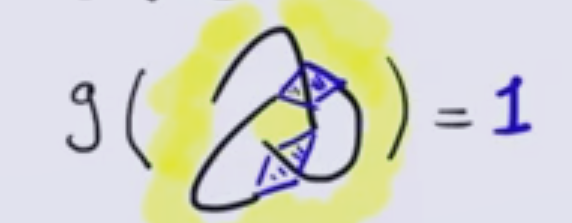
\includegraphics{figures/image_2021-01-18-23-30-49.png}
\caption{The genus of the trefoil}
\end{figure}

\end{exercise}

The genus can be computed by setting
\(\widehat{HFK}(K, a) \coloneqq\bigoplus _m \widehat{HFK}_m(K, a)\),
which yields
\begin{align*}
g(k) = \max \left\{{ a {~\mathrel{\Big|}~}\widehat{HFK}(K, a) \neq 0 }\right\}
.\end{align*}
Note that the \(a\) grading here is referred to as the \textbf{Alexander
grading}.

\end{fact}

\begin{fact}

\(\widehat{HFK}\) detects whether or not a knot is \textbf{fibered},
where \(K\) is fibered if and only if it admits an \(S^1\) family
\(F_t\) of Seifert surfaces such that
\(t\neq s\in S^1 \implies F_t \cap F_s = K\). I.e., there is a fibration
on the knot complement where each fiber is a Seifert surface:

\begin{center}
\begin{tikzcd}
\Sigma_g 
  \ar[r] 
& 
S^3\setminus K
  \ar[d, "\pi"] 
\\
& 
K 
\end{tikzcd}
\end{center}

\begin{example}[The Unknot]

The unknot is fibered by \({\mathbb{D}}^2\)s:

\begin{figure}
\centering
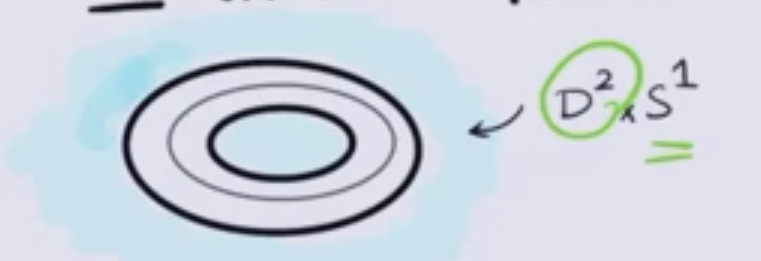
\includegraphics{figures/image_2021-01-18-23-38-35.png}
\caption{The unknot fibered by discs.}
\end{figure}

\end{example}

This is ``detected'' in the following sense: \(K\) is fibered if and
only if
\begin{align*}
\widehat{HFK}(k, g(K)) = {\mathbb{Z}}_2
.\end{align*}

\end{fact}

\begin{definition}[Slice Genus]

Let \(K \subseteq S^3\). We know \(S^3 = {{\partial}}B^4\), so we
consider all of the smoothly properly embedded surfaces \(F\) in \(B^4\)
such that \({{\partial}}F = K\) and take the smallest genus:

\begin{figure}
\centering
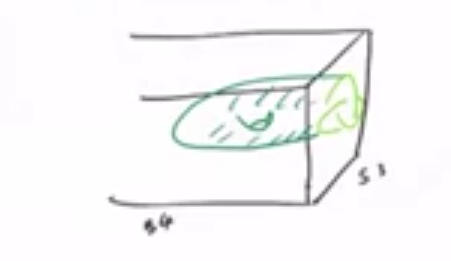
\includegraphics{figures/image_2021-01-18-23-56-35.png}
\caption{Knot in \(S^3\) bounding a surface in \(B^4\)}
\end{figure}

We thus define the \textbf{slice genus} or \textbf{4-ball genus} as
\begin{align*}
g_S(K) \coloneqq g_4(K) \coloneqq\min 
\left\{{
g(F) {~\mathrel{\Big|}~}F\hookrightarrow B^4 \text{ smootherly, properly with } {{\partial}}F = K
}\right\}
.\end{align*}

\end{definition}

\begin{exercise}[?]

Show that \(g_4(K) \leq g(K)\).

\end{exercise}

\begin{definition}[Unknotting number]

Define \(u(K)\) the \textbf{unknotting number} of \(K\) as the minimum
number of times that \(K\) must cross itself to become unknotted.

\end{definition}

\begin{example}[The Trefoil]

Consider changing the bottom crossing of a trefoil:

\begin{figure}
\centering
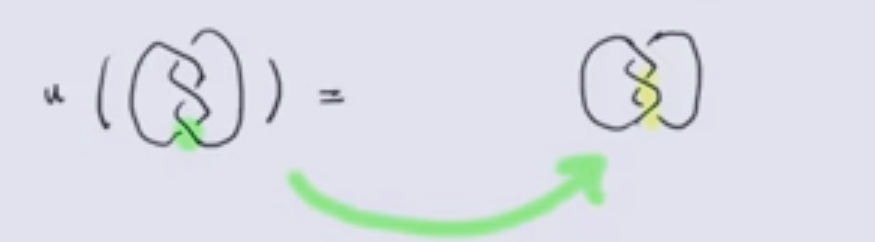
\includegraphics{figures/image_2021-01-19-00-01-14.png}
\caption{Changing one crossing in the trefoil}
\end{figure}

This in fact produces the unknot:

\begin{figure}
\centering
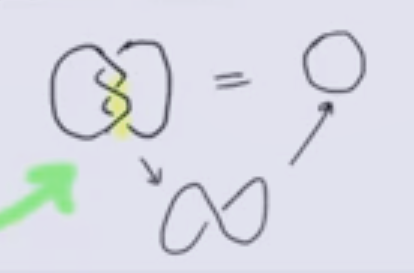
\includegraphics{figures/image_2021-01-19-00-02-00.png}
\caption{Unkink to yield the unknot}
\end{figure}

Thus \(u(K) = 1\), assuming that we know \(K \neq 0\) is not the unknot.

\end{example}

\begin{exercise}[?]

Show that \(g_f(K) \leq u(K)\).

\begin{quote}
Hint: each crossing change \(K\to K'\) yields some surface that is a
cobordism from \(K\) to \(K'\) in \(B^4\), and you can use each step to
build your surface.
\end{quote}

\begin{figure}
\centering
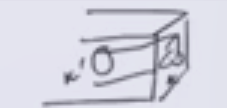
\includegraphics{figures/image_2021-01-19-00-04-13.png}
\caption{Surface between \(K\) and \(K'\)}
\end{figure}

\end{exercise}

\begin{theorem}[Ozsváth-Szabó]

Define an invariant \(\tau(K) \in {\mathbb{Z}}\) from \(\widehat{HFK}\)
such that
\({\left\lvert {\tau(K)} \right\rvert} \leq g_4(K) \leq u(K)\).

\end{theorem}

\begin{definition}[Torus Knots $T_{p, q}$ ]

Recall that we can view
\({\mathbb{T}}^2 \coloneqq{\mathbb{R}}^2/{\mathbb{Z}}^2\) where the
action is \((x, y) \xrightarrow{(m, n)} (x+m, y+m)\), i.e.~we module out
by integer translations. Then for \$p, q \textgreater{} 0 \$ coprime,
\(T_{p, q}\) is the image of the line \(y = mx\) in \({\mathbb{T}}^2\)
where \(m=p/q\).

\end{definition}

\begin{example}[$T_{2, 3}$ ]

The torus knot \(T_{2, 3}\) wraps 3 times around the torus in one
direction and twice in the other:

\begin{figure}
\centering
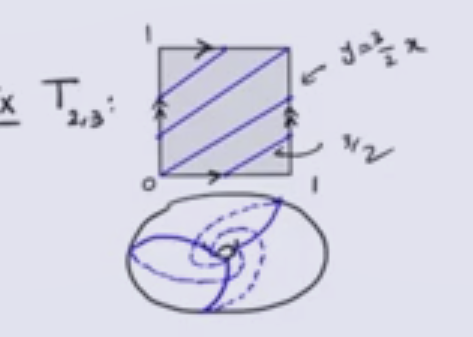
\includegraphics{figures/image_2021-01-19-00-09-51.png}
\caption{The torus knot \(T_{2, 3}\)}
\end{figure}

\end{example}

\begin{theorem}[Milnor]

\begin{align*}
g_4(T_{p, q}) = u(T_{p, q}) = { (p-1)(1-q) \over 2}
.\end{align*}

\begin{itemize}
\tightlist
\item
  First proved by Kronheimer-Mrowka
\item
  Another proof by Osvath-Szabó using Heegard Floer homology.
\end{itemize}

\end{theorem}

\begin{exercise}[?]

Show that \(u(T_{p. q}) \leq {(p-1)(q-1) \over 2}\), i.e.~torus knots
can be unknotted with this many crossing changes.

\end{exercise}

\begin{theorem}[Osvath-Szabó]

\begin{align*}
\tau(T_{p, q}) = 
{(p-1)(q-1) \over 2}
,\end{align*}

which implies
\begin{align*}
{(p-1)(q-1) \over 2}
\leq g_4(T_{p, q})
\leq u(T_{p, q})
\leq {(p-1)(q-1) \over 2}
,\end{align*}
making all of these equal.

\end{theorem}

\begin{remark}

There are better lower bounds for \(u(K)\) defined using
\(\widehat{HFK}\) which are \emph{not} lower bounds for the slice genus.
There are also other lower bounds for the slice genus with different
names (see Jen Hom's survey), some of which are stronger than \(\tau\).

\end{remark}

\begin{remark}

Another application of having these lower bounds is that we can
construct exotic (or \emph{fake}) \({\mathbb{R}}^4\)s, i.e.~4-manifolds
\(X\) homeomorphic to \({\mathbb{R}}^4\) but not diffeomorphic to
\({\mathbb{R}}^4\).

\end{remark}

\begin{remark}

All of these invariants work nicely in a \((3+1){\hbox{-}}\)TQFT: we
have invariants of 3-manifolds \(M_i\) and knots in them, so we can talk
about \textbf{cobordisms} between them: \(W^4\) a compact oriented
4-manifold with \({{\partial}}W^4 = -M_1 {\coprod}M_2\).

\begin{figure}
\centering
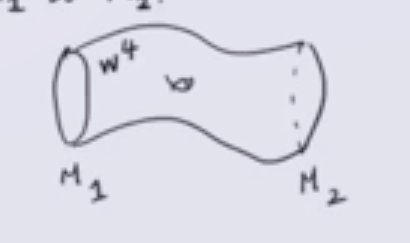
\includegraphics{figures/image_2021-01-19-00-24-31.png}
\caption{A cobordism}
\end{figure}

Osvath-Szabó define a map
\begin{align*}
F_{W, t}^{\,\cdot\,}: HF^{\,\cdot\,}(M_1, { \left.{{t}} \right|_{{M_1}} } ) \to HF^{\,\cdot\,}(M_2, { \left.{{t}} \right|_{{M_2}} })
\end{align*}
using \(t\) coming from the splitting of spin\(^c\) structure which
yields an invariant of closed 4-manifolds referred to as \textbf{mixed
invariants}.

Similarly, if we have knots in 3-manifolds we can define a cobordism
\((M_1, K_1) \to (M_2, K_2)\) as \((W^4, F)\) where \(W^4\) is a
cobordism \(M_1\to M_2\) and \(F\hookrightarrow W\) is a smoothly
embedded surface that is a cobordism from \(K_1\to K_2\) with
\(F \cap M_i = K_i\) and \({{\partial}}F = -K_1 {\coprod}K_2\).

\begin{figure}
\centering
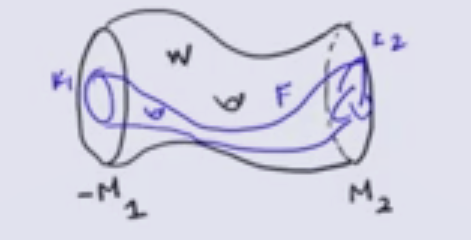
\includegraphics{figures/image_2021-01-19-00-29-04.png}
\caption{A cobordism including knots}
\end{figure}

This similarly yields a map

\begin{align*}
F_{W, F t}^{\,\cdot\,}: HF^{\,\cdot\,}(M_1, K_1, { \left.{{t}} \right|_{{M_1}} } ) \to HF^{\,\cdot\,}(M_2, K_2, { \left.{{t}} \right|_{{M_2}} })
\end{align*}

\end{remark}

\begin{remark}

This smoothly embedded surface in the middle can be used to study other
smoothly embedded surfaces in 4-manifolds, which has been done recently.

\end{remark}

\hypertarget{lecture-2-tuesday-january-19}{%
\section{Lecture 2 (Tuesday, January
19)}\label{lecture-2-tuesday-january-19}}

\todo[inline]{Copy in references recommended by Akram!}

\begin{remark}

For Morse Theory, there are some good exercises in Audin's book --
essentially anything other than the existence questions. The first 8
look good on p.~18.

\end{remark}

Today:

\begin{enumerate}
\def\labelenumi{\arabic{enumi}.}
\item
  Overview of the construction of HF, and
\item
  A discussion of Morse Theory.
\end{enumerate}

\hypertarget{constructing-heegard-floer}{%
\subsection{Constructing Heegard
Floer}\label{constructing-heegard-floer}}

First goal: discuss how the name ``Heegard'' fits in.

\begin{definition}[Genus $g$ handlebody]

A \textbf{genus \(g\) handlebody} \(H_g\) is a compact oriented
3-manifold with boundary obtained from \(B^3\) by attaching \(g\) solid
handles (a neighborhood of an arc).

\end{definition}

\begin{example}[Attaching $g=2$ handles to a sphere]

For \(g=2\) attached to a sphere, we glue \(D^2 \times I\) by its
boundary to \(S^2\).

\begin{figure}
\centering
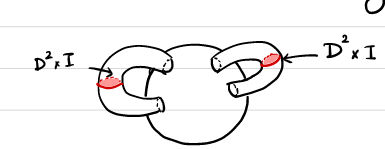
\includegraphics{figures/image_2021-01-19-00-35-48.png}
\caption{image\_2021-01-19-00-35-48}
\end{figure}

In general, \({{\partial}}H_g = \Sigma_g\) is a genus \(g\) surface, and
\(H_g \setminus{\coprod}_{i=1}^g D_i = B^3\). We can keep track of the
data by specifying \((\Sigma, \alpha_1, \alpha_2, \cdots, \alpha_g)\)
where \({{\partial}}D_i = \alpha_i\).

\begin{figure}
\centering
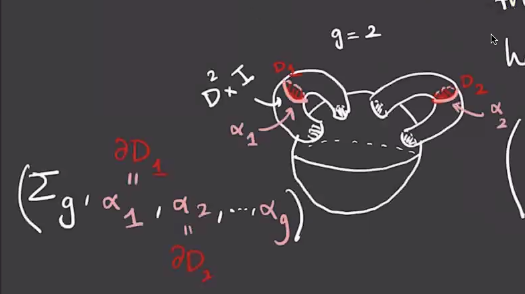
\includegraphics{figures/image_2021-01-19-11-26-35.png}
\caption{Attaching a handlebody}
\end{figure}

\end{example}

\begin{definition}[Heegard Decomposition]

A \textbf{Heegard diagram} is \(M = H_1 \cup_{{\partial}}H_2\) where
\(H_i\) are genus \(g\) handlebodies and there is a diffeomorphism
\({{\partial}}H_1 \to {{\partial}}H_2\).

\end{definition}

\begin{theorem}[?]

Every closed 3-manifold has a Heegard decomposition, although it is not
unique.

\end{theorem}

\begin{definition}[Heegard Diagram]

A \textbf{Heegard diagram} is the data
\((\Sigma_g, \alpha = \left\{{ \alpha_1, \cdots, \alpha_g}\right\}, \beta = \left\{{ \beta_1, \cdots, \beta_g}\right\})\)
where the \(\alpha\) correspond to \(H_1\) and \(\beta\) to \(H_2\) and
\(\Sigma_g = {{\partial}}H_1 = {{\partial}}H_2\).

\end{definition}

\hypertarget{lagrangian-floer-homology}{%
\subsection{Lagrangian Floer Homology}\label{lagrangian-floer-homology}}

This is essentially an infinite-dimensional version of Morse homology.

\begin{definition}[Symplectic Manifold]

A \textbf{symplectic manifold} is a pair \((M^{2n}, \omega)\) such that

\begin{itemize}
\tightlist
\item
  \(\omega\) is \emph{closed}, i.e.~\(d \omega = 0\), and
\item
  \(\omega\) is \emph{nondegenerate}, i.e.~\(\wedge^n \omega \neq 0\).
\end{itemize}

\end{definition}

\begin{definition}[Lagrangian]

A \textbf{Lagrangian submanifold} is an \(L^n \subseteq M\) such that
\({ \left.{{\omega}} \right|_{{L}} } = 0\).

\end{definition}

If \(L_1 \cap L_2\) is finitely many points, case we can define a chain
complex
\begin{align*}
CF(M^{2n}, L_1, L_2) \coloneqq{\mathbb{Z}}_2[L_1 \cap L_2]
,\end{align*}
the \({\mathbb{Z}}_2{\hbox{-}}\)vector space generated by the
intersection points of the Lagrangian submanifolds. We'll define a
differential by essentially counting discs between intersection points:

\begin{figure}
\centering
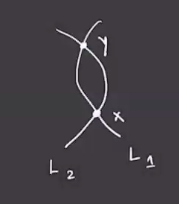
\includegraphics{figures/image_2021-01-19-11-46-38.png}
\caption{Two intersection points}
\end{figure}

We'll want to write \({{\partial}}x = c_y y + \cdots\) where \(c_y\) is
some coefficient. How do we compute it? In this case, we have half of
the boundary on \(L_1\) and half is on \(L_2\)

\begin{figure}
\centering
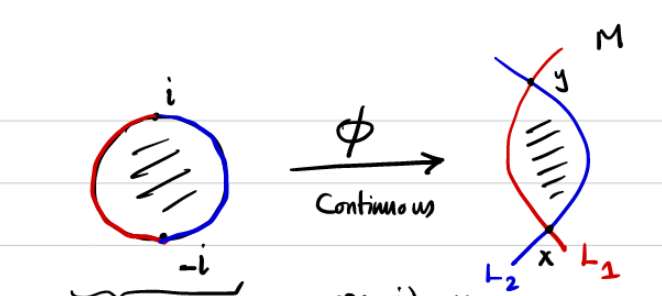
\includegraphics{figures/image_2021-01-19-00-40-08.png}
\caption{i}
\end{figure}

So we can the number of \emph{holomorphic} discs from \(x\) to \(y\).
We'll get
\({\partial}^2 = 0 \iff \operatorname{im}{\partial}\subset \ker {\partial}\),
and \(HF\) will be kernels modulo images. In more detail, we'll have
\begin{align*}
{{\partial}}x = \sum_y \sum_{\mu(\varphi) = 1} \# \widehat{\mathcal{M}} (\varphi)y &&  \widehat{\mathcal{M}}(\varphi) = \mathcal{M}(\varphi) / {\mathbb{R}}
\end{align*}
where \(\widehat{\mathcal{M}}\) will (in good cases) be a 1-dimensional
manifold with finitely many points. Note that it's not necessarily true
that \(CF\) has a grading!

Given a 3-manifold \(M^3\), we'll associate a Heegard diagram
\(\Sigma, \alpha, \beta\). Note the \(g{\hbox{-}}\)element symmetric
group acts on \(\prod_{i=1}^g \Sigma\) by permuting the \(g\)
coordinates, so we can define
\(\operatorname{Sym}^g(\Sigma) \coloneqq\prod_{i=1}^g \Sigma / S_g\).

\begin{theorem}[?]

The space \(\operatorname{Sym}^g(\Sigma)\) is a smooth complex manifold
of \({\mathbb{R}}{\hbox{-}}\)dimension \(2g\).

\end{theorem}

Write
\({\mathbb{T}}_{\alpha} \coloneqq\prod_{i=1}^g \alpha_i \subseteq \prod_{i=1}^g \Sigma\)
for a \(g{\hbox{-}}\)dimensional torus; this admits a quotient map to
\(\operatorname{Sym}^g(\Sigma)\). We can repeat this to obtain
\({\mathbb{T}}_{\beta}\). Then \(HF^{\,\cdot\,}(M)\) will be a variation
of Lagrangian Floer Homology for
\((\operatorname{Sym}^g(\Sigma), {\mathbb{T}}_{\alpha}, {\mathbb{T}}_{\beta} )\).

\begin{example}[?]

Consider constructing a genus \(g=1\) Heegard diagram. Recall that
\(S^3\) can be constructed by gluing two solid torii.

\begin{figure}
\centering
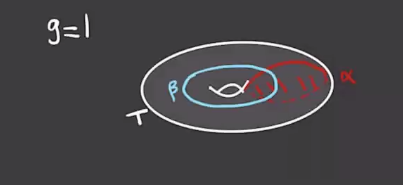
\includegraphics{figures/image_2021-01-19-12-20-16.png}
\caption{image\_2021-01-19-12-20-16}
\end{figure}

Here \((T, \alpha, \beta)\) will be a Heegard diagram for \(S^3\).

\end{example}

\begin{exercise}[?]

Show that the following diagram with \(\beta\) defined as some
perturbation of \(\alpha\) is a Heegard diagram for \(S^1 \times S^2\).

\begin{figure}
\centering
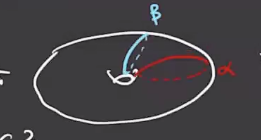
\includegraphics{figures/image_2021-01-19-12-21-56.png}
\caption{image\_2021-01-19-12-21-56}
\end{figure}

\end{exercise}

\begin{definition}[Dehn Surgery]

Consider \(M\) a 3-manifold containing a knot \(K\), we can construct a
new 3-manifold by first removing a neighborhood of \(K\) to yield
\(M\setminus N(K)\):

\begin{figure}
\centering
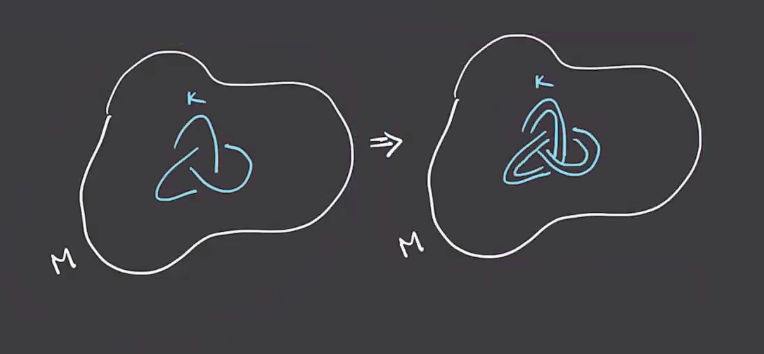
\includegraphics{figures/image_2021-01-19-12-23-16.png}
\caption{image\_2021-01-19-12-23-16}
\end{figure}

Taking a new solid torus \(S \coloneqq{\mathbb{D}}^2 \times S^1\) and a
diffeomorphism \(i: {{\partial}}S \to {{\partial}}(M \setminus N(K))\),
this yields a new manifold \(M _{\varphi} (K)\), a \textbf{surgery}
along \(K\).

\begin{figure}
\centering
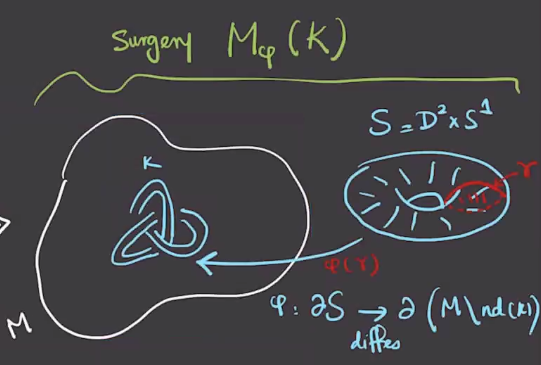
\includegraphics{figures/image_2021-01-19-12-25-25.png}
\caption{image\_2021-01-19-12-25-25}
\end{figure}

\end{definition}

\begin{remark}

Note that the diffeomorphism is entirely determined by the image of the
curve \(\alpha\) . The Knot Floer chain complex of \(K\) will allow us
to compute any flavor \(HF^{\,\cdot\,}M _{\varphi} (K)\) of Floer
homology. Why is this important: any closed 3-manifold is surgery on a
link in \(S^3\). However there are many more computational tools
available here and not in the other theories: combinatorial approaches
to compute, exact sequences, bordered Floer homology.

\end{remark}

Next time: we'll talk about ``integer surgeries''.

\hypertarget{lecture-3-morse-theory-thursday-january-19}{%
\section{Lecture 3: Morse Theory (Thursday, January
19)}\label{lecture-3-morse-theory-thursday-january-19}}

\hypertarget{intro-to-morse-theory}{%
\subsection{Intro to Morse Theory}\label{intro-to-morse-theory}}

Let \(M^n\) be a smooth closed manifold, then the goal is to study the
topology of \(M\) by studying smooth functions
\(f \in C^ \infty (M, {\mathbb{R}})\). We'll need \(f\) to be
\emph{generic} in a sense we'll discuss later.

\begin{definition}[Critical Point]

A point \(p\in M\) is called a \textbf{critical point} if and only if
\((df)_p = 0\).

\end{definition}

\begin{definition}[Hessian / Second Derivative]

Fixing a critical point \(p\) for \(f\), the \textbf{second derivative}
or \textbf{Hessian} of \(f\) at \(p\) is a bilinear form on \(T_pM\)
which is defined in the following way: for \(v, w\in T_p M\), extend
\(w\) to a vector field \(\tilde w\) in a neighborhood of \(p\) and set
\begin{align*}
d^2 f_p(v, w) = v\cdot (\tilde w \cdot f)(p) \coloneqq v \cdot (df)(\tilde w)(p)
.\end{align*}
where we take the derivative of \(f\) with respect to \(\tilde w\), then
take the derivative with respect to \(v\), then evaluate at the point to
get a number.

\end{definition}

\begin{remark}

This is only well-defined at critical points (check!). Note that we need
\(\tilde w\) so that \(\tilde w \cdot f\) is again a function (and not a
number) which can be differentiated again. You can also take
e.g.~\(\tilde v \cdot (\tilde w \cdot f)\), differentiating with respect
to the vector field instead of just the vector \(v\), but we're plugging
in \(p\) in either case.

\end{remark}

\begin{claim}

The second derivative is

\begin{enumerate}
\def\labelenumi{\arabic{enumi}.}
\item
  Well-defined, and
\item
  Symmetric
\end{enumerate}

\end{claim}

\begin{remark}

If you fix a coordinate chart in a neighborhood of \(p\), then the
bilinear form is represented by a matrix given by
\begin{align*}
(d^2 f)_p = H_p =  \qty{ {\frac{\partial ^2}{\partial x_j {\partial}x_i}\,}(p)}_{ij}
.\end{align*}

\end{remark}

\begin{proof}[of 2]

We can compute
\begin{align*}
(d^2 f)_p(v, w) - (d^2 f)_p(w, v) 
&= v\cdot (\tilde w \cdot f)(p) - w \cdot (\tilde v \cdot f)(p) \\
&\coloneqq df_p \qty{ [\tilde v, \tilde w]} \\
& = 0 && \text{since $p$ is a critical point and $df_p = 0$}
.\end{align*}

\end{proof}

\begin{proof}[of 1]

This is now easier to prove: we are picking an extension of \(w\) to a
vector field, so we need to show that the definition doesn't depend on
that choice.
\begin{align*}
(d^2 f)(_p(v, w) 
&= v\cdot (\tilde w \cdot f)(p) && \text{which doesn't depend on }\tilde v\\
&= (d^2 f)_p(w, v) \\
&= w\cdot (\tilde v \cdot f)(p) && \text{which doesn't depend on } \tilde w
,\end{align*}
and thus this is independent of both \(\tilde v\) and \(\tilde w\).

\end{proof}

\begin{exercise}[?]

Show that the second derivative in local coordinates is given by the
matrix \(H_p\) above.

\end{exercise}

\begin{remark}

In local coordinates, we can write
\(v = \sum_{i=1}^n a_i {\frac{\partial }{\partial x_i}\,}\) and
\(w = \sum_{i=1}^n b_i {\frac{\partial }{\partial x_i}\,}\), and thus
\begin{align*}
(d^2 f)_p(v, w) = \mathbf{b}^t H_p \mathbf{a} = \sum_{1 \leq i,j \leq n} a_i b_j {\frac{\partial ^2 f}{\partial x_i {\partial}x_j}\,}(p)
.\end{align*}

\end{remark}

\begin{definition}[Nondegenerate Critical Points]

A critical point \(p\in M\) is called \textbf{nondegenerate} if the
bilinear form \((d^2 f)_p\) is nondegenerate at \(p\), i.e.~for all
\(v\in T_p M\) there exists a
\(w\in T_pM\setminus\left\{{\mathbf{0}}\right\}\) such that
\((d^2 f)_p(v, w) \neq 0\). This occurs if and only if \(H_p\) is
invertible.

\end{definition}

\begin{definition}[Index of a critical point]

Given a nondegenerate critical point \(p\in M\), define the
\textbf{index} \(\mathop{\mathrm{Ind}}(p)\) of \(f\) at \(p\) in the
following way: since \(H_p\) is symmetric and nondegenerate, its
eigenvalues are real and nonzero, so define the index as the number of
\emph{negative} eigenvalues of \(H_p\).

\end{definition}

\begin{definition}[Morse Function]

A function \(f\in C^ \infty (M, {\mathbb{R}})\) is called a
\textbf{Morse function} if and only if all of its critical points are
nondegenerate.

\end{definition}

\begin{remark}

We'll see that almost every smooth function is Morse, and these are
preferable since they have a simple and predictable structure near
critical points and don't do anything interesting elsewhere.

\end{remark}

\begin{theorem}[Morse Lemma]

Let \(p\in M\) be a nondegenerate critical point of \(f\) with
\(\mathop{\mathrm{Ind}}(p) = \lambda\). Then there exists charts
\(\varphi:(U, p) \to ({\mathbb{R}}^n, 0)\) such that writing \(f\) in
local coordinates yields
\begin{align*}
(f \circ \varphi ^{-1} )(x) = f(p) - \sum_{i=1}^{\lambda} x_i^2 + \sum_{j= \lambda + 1}^n x_j^2
.\end{align*}

\end{theorem}

\begin{remark}[Observation 1]

We have
\begin{align*}
H_p = 
\begin{bmatrix}
-2&&&&&&\\
&\ddots&&&&&\\
&&-2&&&&\\
&&&2&&&\\
&&&&\ddots&&\\
&&&&&2&\\
&&&&&&2
\end{bmatrix}
= -2 I_{\lambda} \oplus 2 I_{n- \lambda}
.\end{align*}

\end{remark}

\begin{remark}[Observation 2]

If \(\lambda=n\)??

\end{remark}

\begin{remark}[Observation 3]

??

\end{remark}

\begin{example}[Sphere]

Consider \(S^2\) with a height function:

\begin{figure}
\centering
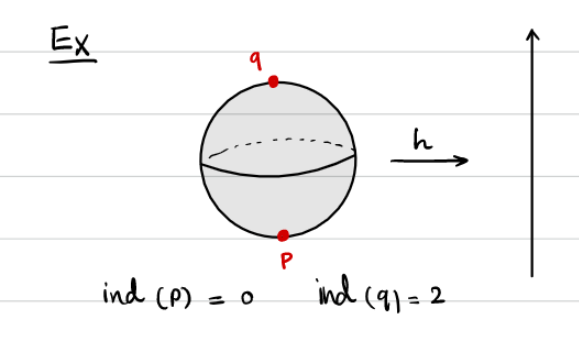
\includegraphics{figures/image_2021-01-19-00-49-32.png}
\caption{Sphere with a height function}
\end{figure}

Then we have a local minimum at the South pole \(p\) and a local max at
the North pole \(q\), where \(\mathop{\mathrm{Ind}}(p) = 0\) and
\(\mathop{\mathrm{Ind}}(q) = 2\). Note that the critical points
essentially occur where the tangent space is horizontal

\end{example}

\begin{example}[Torus]

Consider \({\mathbb{T}}^2\) with the height function:

\begin{figure}
\centering
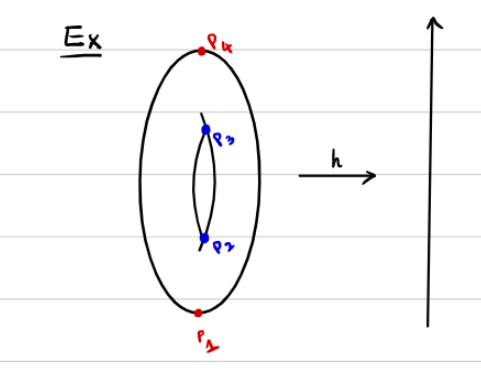
\includegraphics{figures/image_2021-01-19-00-49-53.png}
\caption{Torus with a height function}
\end{figure}

This has a similar max/min as the sphere, but also has two critical
points in the middle that resemble saddles:

\begin{figure}
\centering
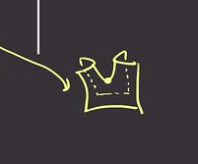
\includegraphics{figures/image_2021-01-21-12-04-50.png}
\caption{Saddle points}
\end{figure}

\end{example}

\begin{remark}

Define \(M_a \coloneqq f ^{-1} ((- \infty , a])\); we then want to
consider how \(M_a\) changes as \(a\) changes:

\begin{figure}
\centering
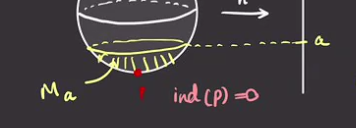
\includegraphics{figures/image_2021-01-21-12-06-29.png}
\caption{\(M_a\) on the sphere}
\end{figure}

\begin{figure}
\centering
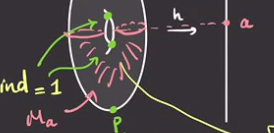
\includegraphics{figures/image_2021-01-21-12-06-49.png}
\caption{\(M_a\) on the torus}
\end{figure}

\end{remark}

\begin{lemma}[?]

If \(f ^{-1} ([a, b])\) contains no critical points, then
\begin{align*}
f ^{-1} (a) &\cong f ^{-1} (b) \\
M_a &\cong M_b
.\end{align*}

\end{lemma}

\begin{definition}[Gradients]

Choose a metric \(g\) on \(M\), then the \textbf{gradient vector} of
\(f\) is given by
\begin{align*}
g(\nabla f, v) = df(v)
.\end{align*}

\end{definition}

\begin{remark}

We have
\begin{align*}
df( \nabla f) = g(\nabla f, \nabla f) = {\left\lVert {\nabla f} \right\rVert}^2
.\end{align*}

\end{remark}

\begin{proof}[?]

We have the following situation:

\begin{figure}
\centering
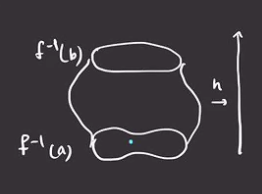
\includegraphics{figures/image_2021-01-21-12-11-16.png}
\caption{image\_2021-01-21-12-11-16}
\end{figure}

The gradient vector is always tangent to the level sets, so we can
consider the curve \(\gamma\) which satisfies
\(\dot\gamma(t) = -\nabla f( \gamma(t))\):

\begin{figure}
\centering
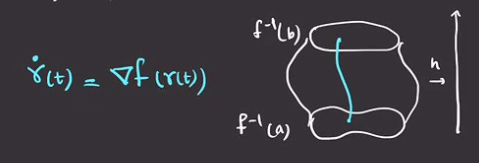
\includegraphics{figures/image_2021-01-21-12-12-42.png}
\caption{image\_2021-01-21-12-12-42}
\end{figure}

For technical reasons, we want to end up with cohomology instead of
homology and will take \(-\nabla f\) instead of \(\nabla f\) everywhere:

\begin{figure}
\centering
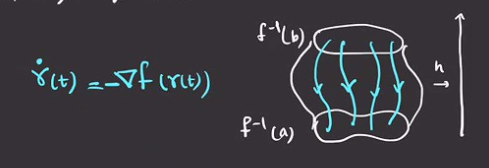
\includegraphics{figures/image_2021-01-21-12-13-35.png}
\caption{image\_2021-01-21-12-13-35}
\end{figure}

So \(\gamma\) will be a trajectory of \(- \nabla f\), and
\(f ^{-1} [a, b] \cong f ^{-1} (a) \times[0, 1]\). A problem is that
following these trajectories may involve arriving at \(f ^{-1} (a)\) at
different times:

\begin{figure}
\centering
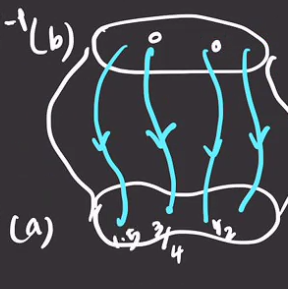
\includegraphics{figures/image_2021-01-21-12-15-10.png}
\caption{image\_2021-01-21-12-15-10}
\end{figure}

We can fix this by normalizing:
\begin{align*}
V \coloneqq- \nabla f / {\left\lVert { \nabla f} \right\rVert}^2 \implies (df)(v) = {\left\langle { \nabla f},~{ - \nabla f / {\left\lVert {\nabla f} \right\rVert}^2} \right\rangle} = -1
.\end{align*}

For every \(p \in f ^{-1} (b)\), if \(\gamma(t)\) is the trajectory
starting from \(p\), i.e.~\(\gamma(0) = p\), then
\(\gamma(b-a) \in f ^{-1} (a)\). So define
\begin{align*}
\Phi: f ^{-1} (b) \times[0, b-a] &\to f ^{-1} ([a, b]) \\
(p, t) &\mapsto \gamma_p (t)
,\end{align*}
which will be a diffeomorphism.

\end{proof}

\begin{theorem}[?]

Suppose \(f ^{-1} ([a, b])\) contains exactly one critical point \(p\)
with \(\mathop{\mathrm{Ind}}(p) = \lambda\) and \(f(p) = c\). Then
\begin{align*}
M_b = M_a \cup_{{{\partial}}} \qty{ D^ \lambda \times D^{n - \lambda} }
\end{align*}
where \(n \coloneqq\dim M\).

\end{theorem}

\begin{example}[?]

For \(\lambda= 1, n - \lambda= 2\):

\begin{figure}
\centering
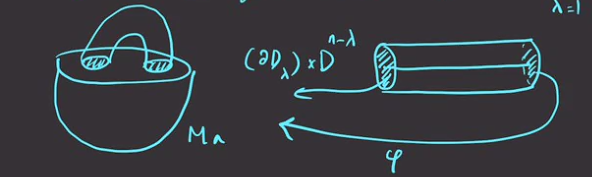
\includegraphics{figures/image_2021-01-21-12-32-38.png}
\caption{image\_2021-01-21-12-32-38}
\end{figure}

\end{example}

\begin{example}[?]

\begin{figure}
\centering
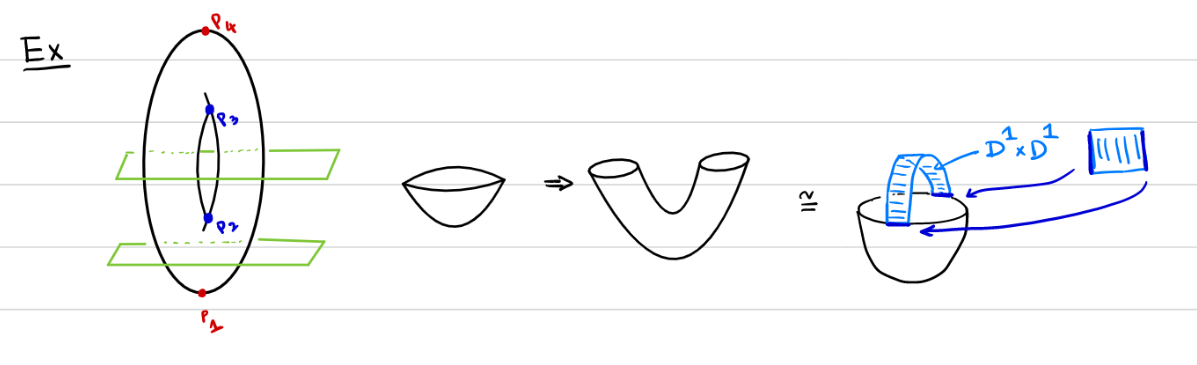
\includegraphics{figures/image_2021-01-19-00-53-07.png}
\caption{image\_2021-01-19-00-53-07}
\end{figure}

\end{example}

\begin{definition}[Unstable Submanifold]

\begin{align*}
W_f^u(p) \coloneqq\left\{{p}\right\} \cup\left\{{
\dot{\gamma(t)} = -\nabla f(\gamma(t)),\, \lim_{t\to -\infty} \gamma(t) = p,\, t\in {\mathbb{R}}
}\right\}
.\end{align*}

\end{definition}

\begin{lemma}[?]

If \(\mathop{\mathrm{Ind}}(p) = \lambda\) then
\(W_f^u(p) \cong {\mathbb{R}}^ \lambda\).

\end{lemma}

\begin{example}[?]

\begin{figure}
\centering
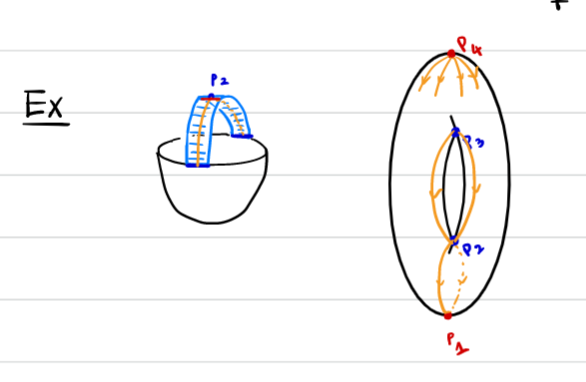
\includegraphics{figures/image_2021-01-19-00-55-24.png}
\caption{image\_2021-01-19-00-55-24}
\end{figure}

\end{example}

\begin{example}[?]

\begin{figure}
\centering
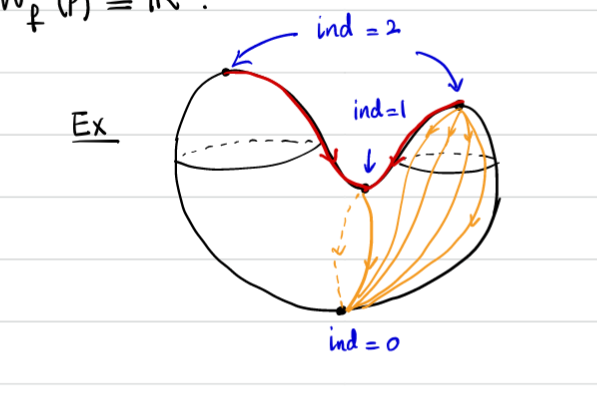
\includegraphics{figures/image_2021-01-19-00-55-41.png}
\caption{image\_2021-01-19-00-55-41}
\end{figure}

\end{example}

\begin{definition}[Stable Manifold]

\begin{align*}
W_f^s(p) \coloneqq\left\{{p}\right\} \cup\left\{{
\dot{\gamma(t)} = -\nabla f(\gamma(t)),\, \lim_{t\to +\infty} \gamma(t) = p,\, t\in {\mathbb{R}}
}\right\}
.\end{align*}

\end{definition}

\begin{lemma}[?]

If \(\mathop{\mathrm{Ind}}(p) = \lambda\) then
\(W_f^s(p) \cong {\mathbb{R}}^{n- \lambda}\).

\end{lemma}

\begin{definition}[$C^\infty$ ]

\(C^ \infty (M; {\mathbb{R}})\) is defined as smooth function
\(M\to |RR\), topologized as:

\begin{itemize}
\tightlist
\item
  ?
\item
  ?
\end{itemize}

And a basis for open neighborhoods around \(p\) is given by
\begin{align*}
N_g(f) = \left\{{
g:M\to {\mathbb{R}}{~\mathrel{\Big|}~}
{\left\lvert {
{\frac{\partial ^k g}{\partial {\partial}x _{i_1} \cdots {\partial}x _{i_k} }\,}(p)
- 
{\frac{\partial ^k f}{\partial {\partial}x _{i_1} \cdots {\partial}x _{i_k} }\,}(p)
} \right\rvert} < \infty\, \forall \alpha,\, \forall p\in h_ \alpha(C_ \alpha)
}\right\}
.\end{align*}

\end{definition}

\begin{theorem}[?]

The set of Morse functions on \(M\) is open and dense in
\(C^ \infty (M; {\mathbb{R}})\).

\end{theorem}

\hypertarget{tuesday-january-26}{%
\section{Tuesday, January 26}\label{tuesday-january-26}}

\hypertarget{attaching-handles}{%
\subsection{Attaching Handles}\label{attaching-handles}}

Goal: we want to use Morse functions (smooth, nondegenerate critical
points) to study the topology of \(M\). Recall that the torus had 4
critical points,

\begin{figure}
\centering
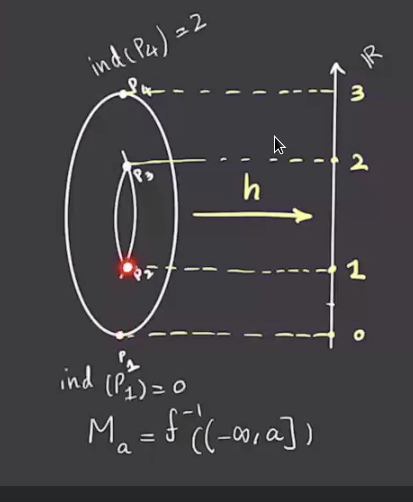
\includegraphics{figures/image_2021-01-26-11-14-32.png}
\caption{image\_2021-01-26-11-14-32}
\end{figure}

We defined the index as the number of negative eigenvalues of the
Hessian matrix. Here the highest index will be the dimension of the
manifold, and by the Morse lemma the two intermediate critical points
will be index 1.

\begin{remark}

We want to use the Morse function to decompose the manifold, so we
consider \(M_a \coloneqq f ^{-1} ((- \infty , a ])\). If
\(f ^{-1} [a, b]\) does not contain a critical point, then
\(M_a \cong M_b\) and \(f ^{-1} (a) \cong f ^{-1} (b)\). So taking
\(M_{1/2}\) and \(M_{3/4}\) here both yield discs:

\begin{figure}
\centering
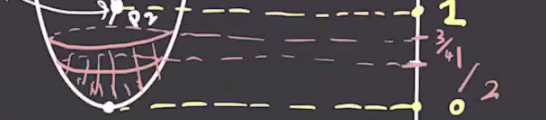
\includegraphics{figures/image_2021-01-26-11-17-46.png}
\caption{image\_2021-01-26-11-17-46}
\end{figure}

Passing through critical points does change the manifold, though:

\begin{figure}
\centering
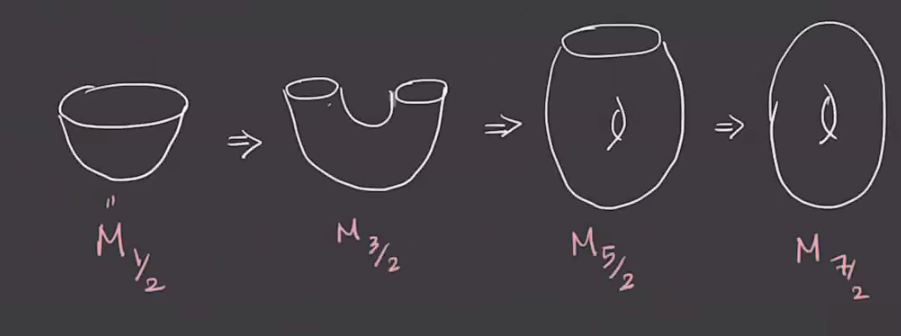
\includegraphics{figures/image_2021-01-26-11-19-01.png}
\caption{image\_2021-01-26-11-19-01}
\end{figure}

\end{remark}

\begin{theorem}[?]

Suppose \(f ^{-1} [a, b]\) contains exactly \emph{one} critical point of
index \(\lambda\) then
\begin{align*}
M_b \cong M_a \cup_{\varphi} (D_ \lambda \times D_{n - \lambda})
,\end{align*}
where
\(\varphi: ({{\partial}}D_ \lambda \times D_{ n - \lambda}) \hookrightarrow{{\partial}}M_a\).

\end{theorem}

\begin{example}[?]

For the case \(\lambda= 1, n = 3\), we have the following situation:

\begin{figure}
\centering
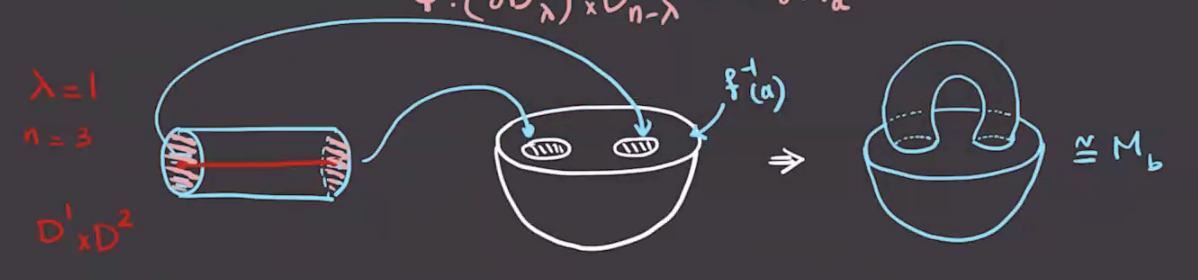
\includegraphics{figures/image_2021-01-26-11-24-46.png}
\caption{image\_2021-01-26-11-24-46}
\end{figure}

\end{example}

\begin{example}[?]

Taking \(\lambda=1, n=2\), we attach \(D^1 \times D^1\) and get the
following situation:

\begin{figure}
\centering
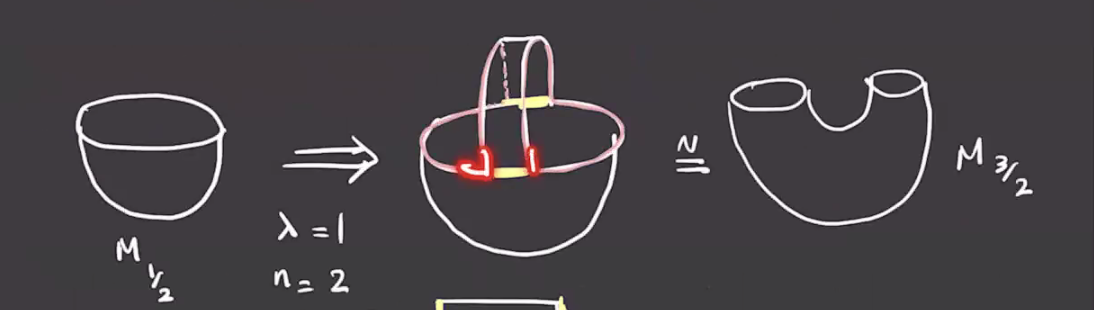
\includegraphics{figures/image_2021-01-26-11-27-16.png}
\caption{image\_2021-01-26-11-27-16}
\end{figure}

Adding on another piece, the new boundary is given by the highlighted
region:

\begin{figure}
\centering
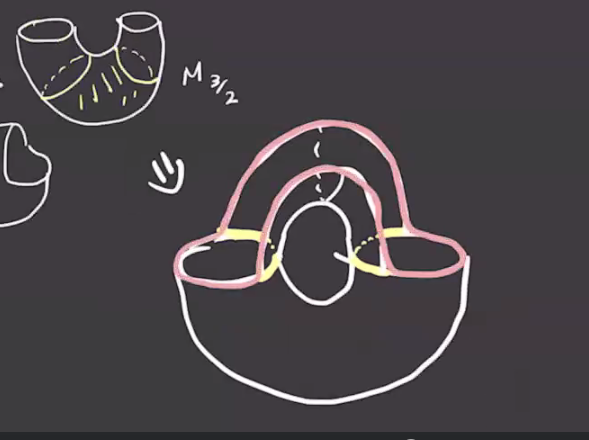
\includegraphics{figures/image_2021-01-26-11-32-27.png}
\caption{image\_2021-01-26-11-32-27}
\end{figure}

And continuing to attach the last pieces yields the following:

\begin{figure}
\centering
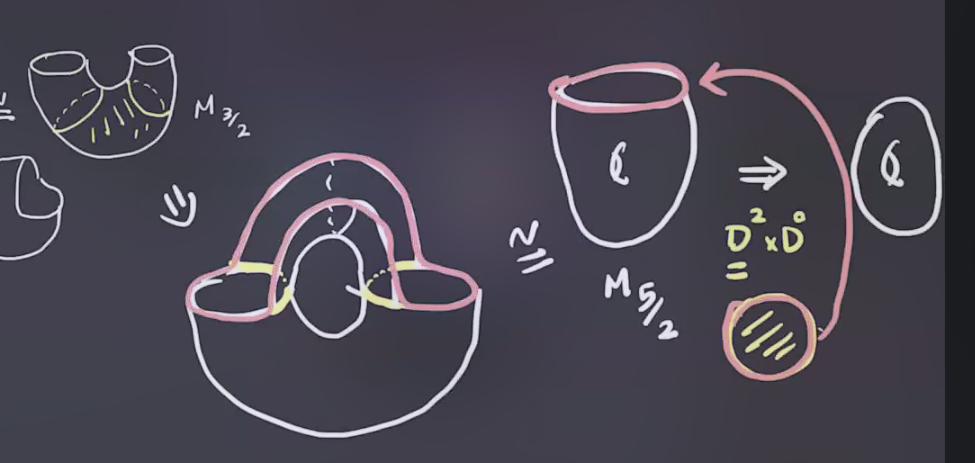
\includegraphics{figures/image_2021-01-26-11-33-31.png}
\caption{image\_2021-01-26-11-33-31}
\end{figure}

\end{example}

\begin{remark}

There is a deformation retract \(M_b \to M_a \cup C_ \lambda\), where
\(C_ \lambda\) is a \(\lambda{\hbox{-}}\)cell given by
\(D_ \lambda \times\left\{{0}\right\}\). For example:

\begin{figure}
\centering
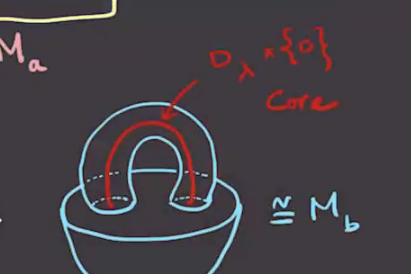
\includegraphics{figures/image_2021-01-26-11-36-35.png}
\caption{image\_2021-01-26-11-36-35}
\end{figure}

\end{remark}

\hypertarget{stable-and-unstable-manifolds}{%
\subsection{Stable and Unstable
Manifolds}\label{stable-and-unstable-manifolds}}

\begin{definition}[Unstable Manifold]

Given \(- \nabla f\) for a fixed metric, the \textbf{unstable manifold}
for a critical point \(p\) is defined as
\begin{align*}
W_f^u(p) \coloneqq\left\{{p}\right\} \cup\left\{{ \gamma(t) {~\mathrel{\Big|}~}\dot \gamma(t) = - \nabla f( \gamma(t) ),\, \gamma(t) \overset{t\to -\infty}\to p }\right\}
.\end{align*}
Here \(\gamma(t)\) is the trajectory of \(-\nabla(f)\).

\end{definition}

\begin{example}[?]

The unstable manifold is highlighted in blue here:

\begin{figure}
\centering
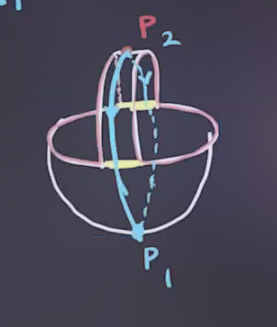
\includegraphics{figures/image_2021-01-26-11-42-01.png}
\caption{image\_2021-01-26-11-42-01}
\end{figure}

The gradient trajectories for other points are given by the yellow lines
in the following:

\begin{figure}
\centering
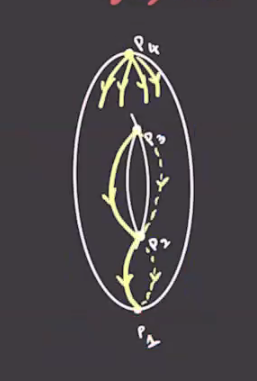
\includegraphics{figures/image_2021-01-26-11-44-13.png}
\caption{image\_2021-01-26-11-44-13}
\end{figure}

\end{example}

\begin{lemma}[?]

If \(\mathop{\mathrm{Ind}}(p) = \lambda\), then the unstable manifold
\(W_f^u\) at \(p\) is isomorphic to \({\mathbb{R}}^ \lambda\).

\end{lemma}

\begin{example}[?]

\begin{figure}
\centering
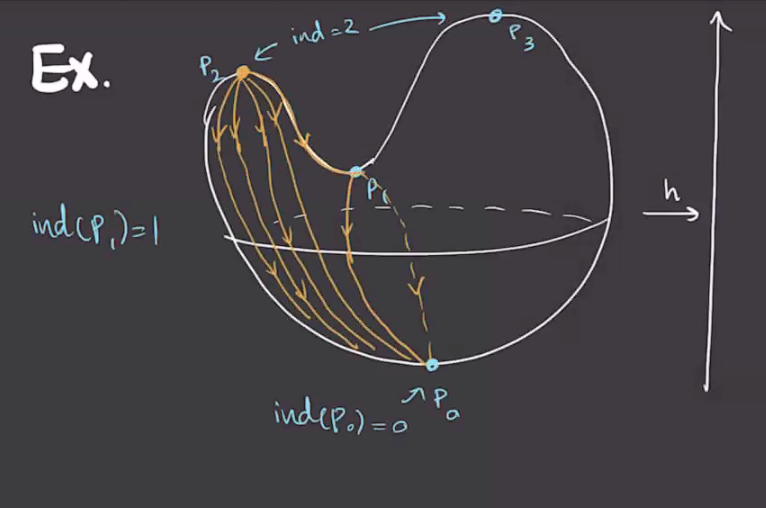
\includegraphics{figures/image_2021-01-26-11-46-46.png}
\caption{image\_2021-01-26-11-46-46}
\end{figure}

Here the unstable manifold for \(p_2\) will be 2-dimensional, with one
flow line ending at \(p_1\) and the rest ending at \(p_0\).

\begin{figure}
\centering
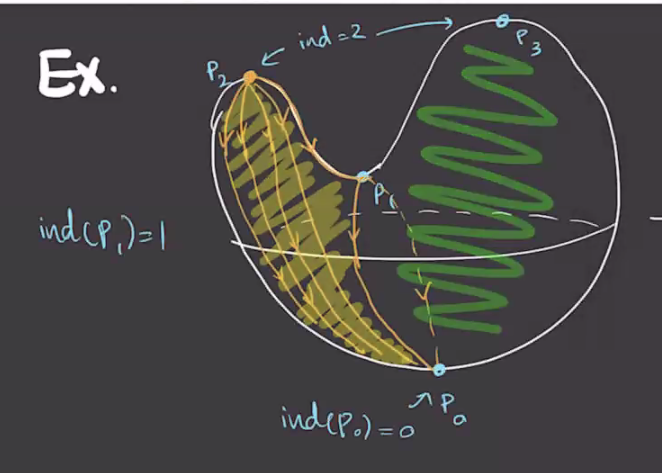
\includegraphics{figures/image_2021-01-26-11-47-24.png}
\caption{image\_2021-01-26-11-47-24}
\end{figure}

\end{example}

\begin{definition}[Stable Manifold]

The \textbf{stable manifold} for a critical point \(p\) is defined as
\begin{align*}
W_f^s(p) \coloneqq\left\{{p}\right\} \cup\left\{{ \gamma(t) {~\mathrel{\Big|}~}\dot \gamma(t) = - \nabla f( \gamma(t) ),\, \gamma(t) \overset{t\to {\color{red} +} \infty}\to p }\right\}
.\end{align*}

\end{definition}

\begin{example}[?]

The stable manifold for \(p_0\) above is every trajectory ending at
\(p_0\). \(W^s(p) = S^2 \setminus W^s(p_1) \cup W_s(p_3)\)? See video?

\todo[inline]{Which point $p$ is this for?}

\end{example}

\hypertarget{morse-functions}{%
\subsection{Morse Functions}\label{morse-functions}}

\begin{theorem}[Existence of Morse Functions]

The set of Morse functions is open and dense in
\(C^ \infty (M; {\mathbb{R}})\) in a certain topology.\footnote{See
  Akram's notes for details.}

\end{theorem}

\begin{remark}

We'll use this to define a chain complex \(C_*(f, g)\) where \(g\) is a
chosen metric, define a differential, and use this to define a homology
theory. For notation, we'll write \(\operatorname{crit}(f)\) as the set
of critical points of \(f\), and given
\(p, q\in \operatorname{crit}(f)\) with \(\gamma\) a trajectory running
from \(p\) to \(q\), we have
\begin{align*}
W^u(p) \cap W^s(q) = \left\{{ \gamma(t) {~\mathrel{\Big|}~}
\gamma(t) \overset{t\to -\infty }\to p,\,
\gamma(t) \overset{t\to +\infty }\to q
}\right\}
.\end{align*}

\end{remark}

\begin{definition}[Transverse Intersections]

Two submanifolds \(X, Y \subseteq M\) \textbf{intersect transversely} if
and only if
\begin{align*}
T_pX + T_p Y \coloneqq\left\{{v+w{~\mathrel{\Big|}~}v\in T_p X, w\in T_p Y}\right\} = T_p M && \forall p\in X \cap Y
.\end{align*}
In this case, we write \(X \pitchfork Y\).

\end{definition}

\begin{example}[?]

An example of a transverse intersection:

\begin{figure}
\centering
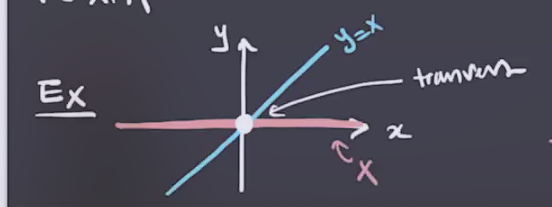
\includegraphics{figures/image_2021-01-26-12-02-29.png}
\caption{image\_2021-01-26-12-02-29}
\end{figure}

\end{example}

\begin{example}[?]

An example of an intersection that is \emph{not} transverse:

\begin{figure}
\centering
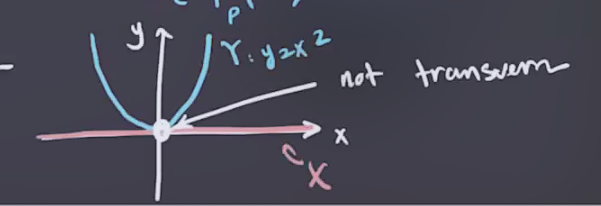
\includegraphics{figures/image_2021-01-26-12-03-13.png}
\caption{image\_2021-01-26-12-03-13}
\end{figure}

\end{example}

\begin{definition}[Morse-Smale]

A pair \((f, g)\) with \(f\) a Morse function and \(g\) a metric is
\textbf{Morse-Smale} if and only if

\begin{itemize}
\tightlist
\item
  \(f\) is a Morse function,
\item
  \(W^u(p)\) is \emph{transverse} to \(W^s(q)\) for all
  \(p, q\in \operatorname{crit}(f)\).
\end{itemize}

\end{definition}

\begin{theorem}[?]

For a generic metric \(g\), the pair \((f, g)\) is Morse-Smale.

\end{theorem}

\begin{remark}

This means that metrics can be perturbed to become Morse-Smale.

\end{remark}

\begin{example}[?]

The following is not Morse-Smale:

\begin{figure}
\centering
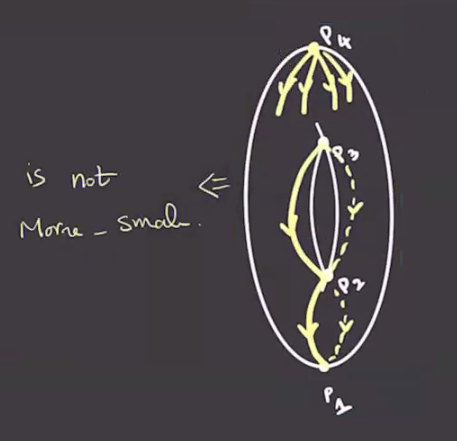
\includegraphics{figures/image_2021-01-26-12-06-06.png}
\caption{image\_2021-01-26-12-06-06}
\end{figure}

Note that if \(X^a \pitchfork Y^b\), then \(X \cap Y \subseteq M^n\) is
a smooth submanifold of dimension \(a+b-n\). In general, we have
\(M^s(p) \cong {\mathbb{R}}^{n - \lambda}\) where
\(\lambda = \mathop{\mathrm{Ind}}(p)\).

\begin{observation}

If \((f, g)\) is Morse-Smale, then \(M^u(p) \pitchfork M^s(q)\). In this
case,
\begin{align*}
\dim(M^u(p) \cap M^s(q)) = \mathop{\mathrm{Ind}}(p) + n - \mathop{\mathrm{Ind}}(q) - n = \mathop{\mathrm{Ind}}(p) - \mathop{\mathrm{Ind}}(q)
.\end{align*}
Thus if \(\mathop{\mathrm{Ind}}(p) = \mathop{\mathrm{Ind}}(q)\) then
\(\dim M^s(p) \cap M^s(q) = 0\).

\end{observation}

\begin{remark}

There is an \({\mathbb{R}}{\hbox{-}}\)action of \(M^s(p) \cap M^s(q)\):
\begin{align*}
\qty{ M^s(p) \times M^u(q) } \times{\mathbb{R}}&\to M^s(p) \cap M^u(q) \\
( \gamma(t), c) &\mapsto \gamma(t+c)
.\end{align*}
If \(p\neq q\), this action is free and we can thus quotient by it to
obtain
\begin{align*}
\mathcal{M}(p, q) \coloneqq\qty{ M^s(p) \cap M^u(q)} / {\mathbb{R}}
.\end{align*}
This identifies all points on the same trajectory, yielding one point
for every trajectory, and so this is called the \textbf{moduli space of
trajectories from \(p\) to \(q\)}.

\end{remark}

If \(\mathop{\mathrm{Ind}}(p) = \mathop{\mathrm{Ind}}(q)\), we have
\(\dim M^u(p) \cap M^s (q) = 0\), making \(\dim \mathcal{M}(p, q) = -1\)
and thus \(\mathcal{M}(p, q) = \emptyset\) and no gradient trajectories
connect \(p\) to \(q\). Referring back to the example, since
\(\mathop{\mathrm{Ind}}(p_3) = \mathop{\mathrm{Ind}}(p_2)\), if
\((f, g)\) were Morse-Smale then there would be no trajectory
\(p_3 \to p_2\), whereas in this case there is at least one.

\end{example}

\begin{remark}

If \(\mathop{\mathrm{Ind}}(p) - \mathop{\mathrm{Ind}}(q) = 1\), then
\(\dim \mathcal{M}(p, q) = \mathop{\mathrm{Ind}}(p) - \mathop{\mathrm{Ind}}(q) - 1 = 0\),
making \(\mathcal{M}(p, q)\) a compact 0-dimensional manifold, which is
thus finitely many points, meaning there are only finitely many
trajectories connecting \(p\to q\) and it becomes possible to define a
Morse complex.

\end{remark}

\begin{definition}[Morse Complex]

Fix \((f, g)\) a Morse-Smale pair, then define
\begin{align*}
C_i(f, g) \coloneqq{\mathbb{Z}}/2{\mathbb{Z}}\left[\left\{{p {~\mathrel{\Big|}~}\mathop{\mathrm{Ind}}p = i}\right\}\right] = \bigoplus_{\mathop{\mathrm{Ind}}(p) = i} {\mathbb{Z}}/2{\mathbb{Z}}\left\langle{p}\right\rangle
,\end{align*}
with a differential
\begin{align*}
{{\partial}}: C_i(f, g) &\to C_{i-1}(f, g) \\
p, \mathop{\mathrm{Ind}}(p) = i & \mapsto \sum_{\mathop{\mathrm{Ind}}(q) = i-1} \# \mathcal{M}(p, q) q 
,\end{align*}
where we take the count mod 2.

\end{definition}

\begin{theorem}[?]

\({{\partial}}^2 = 0\), and thus \(( C(f, g), {{\partial}})\) is a chain
complex.

\end{theorem}

Next time we will work on proving this.

\hypertarget{morse-homology-and-lagrangian-floer-homology-thursday-january-28}{%
\section{Morse Homology and Lagrangian Floer Homology (Thursday, January
28)}\label{morse-homology-and-lagrangian-floer-homology-thursday-january-28}}

\hypertarget{morse-homology}{%
\subsection{Morse Homology}\label{morse-homology}}

Last time: defined the Morse complex. Assumed \((f, g)\) was a
Morse-Smale pair, where \(f\) is a Morse function and \(g\) is a
Riemannian metric, and this guarantees that if
\(p, q\in \operatorname{crit}(f)\) with
\(\mathop{\mathrm{Ind}}(p) - \mathop{\mathrm{Ind}}(q) = 1\), then (among
other things) there are finitely many gradient trajectories
\(p\leadsto q\). We denoted this \(\mathcal{M}(p, q)\). The chain
complex was defined by
\(C_i(f, g) \coloneqq\bigoplus_{\mathop{\mathrm{Ind}}(p) = i} {\mathbb{Z}}_2 \left\langle{ p }\right\rangle\)
with differential \({{\partial}}_i: C_i \to C_{i-1}\) was defined by
sending an index \(i\) critical point \(p\) to
\(\sum_{\mathop{\mathrm{Ind}}(q) = i-1} \# \mathcal{M}(p, q) q \pmod 2\).

\begin{theorem}[The Morse Complex is a Chain Complex]

\({{\partial}}_{i} \circ {{\partial}}_{i+1} = 0\).

\end{theorem}

\begin{proof}[?]

Idea of the proof: we can directly compute
\begin{align*}
{{\partial}}({{\partial}}p) 
&= {{\partial}}\qty{ \sum_{\mathop{\mathrm{Ind}}(q) = i-1} \# \mathcal{M}(p, q) q } \\
&= \sum_{\mathop{\mathrm{Ind}}(q) = i-1} \# \mathcal{M}(p, q) {{\partial}}q \\
&= \sum_{\mathop{\mathrm{Ind}}(q) = i-1} \# \mathcal{M}(p, q) \qty{ \sum_{\mathop{\mathrm{Ind}}(r) = i-2 \# \mathcal{M}(q, r) r  }}   \\
&= \sum_{\mathop{\mathrm{Ind}}(r) = i-2} \qty{\sum_{\mathop{\mathrm{Ind}}(q) = i-1} \# \mathcal{M}(p, q) \# \mathcal{M}(q, r) }  r \\
&= \sum_{\mathop{\mathrm{Ind}}(r) = i-2} c_{p,q,r} r \\
&= 0 && \text{(claim)}
.\end{align*}

This happens if and only if \(c_{p, q, r} = 0 \pmod 2\) for all \(r\)
with \(\mathop{\mathrm{Ind}}(r) = i-2\). This is multiplication of the
number of trajectories:

\begin{figure}
\centering
\includegraphics{figures/image_2021-01-28-11-23-19.png}
\caption{image\_2021-01-28-11-23-19}
\end{figure}

In other words, this is the total number of trajectories \(p\leadsto r\)
that pass through \(q\). These trajectories ``break'' at \(q\), and so
we refer to these as \textbf{broken trajectories}.

\end{proof}

\begin{definition}[Broken Trajectories]

Suppose \(\mathop{\mathrm{Ind}}(r) = \mathop{\mathrm{Ind}}(p) - 2\),
then a \textbf{broken trajectory} from \(p\) to \(r\) is a trajectory
from \(p\) to \(q\) followed by a trajectory \(q\) to \(r\) where
\(\mathop{\mathrm{Ind}}(q) = \mathop{\mathrm{Ind}}(p)-1 = \mathop{\mathrm{Ind}}(r) + 1\).

\begin{figure}
\centering
\includegraphics{figures/image_2021-01-28-11-26-25.png}
\caption{image\_2021-01-28-11-26-25}
\end{figure}

\end{definition}

\begin{question}

Why is the number of broken trajectories even?

\end{question}

\begin{answer}

We can check that
\(\dim \mathcal{M}(p, r) = \dim \qty{ W^u(p) \pitchfork W^s(r)}/{\mathbb{R}}= (\mathop{\mathrm{Ind}}(p) - \mathop{\mathrm{Ind}}(r)) - 1 = 2-1 = 1\).
We can compactify \(\mathcal{M}(p, r)\) by adding in all of the broken
trajectories to define
\begin{align*} 
\overline{\mathcal{M}(p, r)} \cup\qty{ \bigcup_{\mathop{\mathrm{Ind}}(q) = i-1} \mathcal{M}(p, q) \times\mathcal{M}(q, r) } 
.\end{align*}
This is useful here because we can appeal to the classification of
smooth compact 1-dimensional manifolds, which are unions of copies of
\(S^1\) and \(D_1 = I\). In particular, the number of boundary points
\begin{align*}
{{\partial}}\overline{\mathcal{M}(p, r)} = \bigcup_{\mathop{\mathrm{Ind}}(q) = i-1} \mathcal{M}(p, q) \times\mathcal{M}(q, r)
\end{align*}
is even:

\begin{figure}
\centering
\includegraphics{figures/image_2021-01-28-11-32-34.png}
\caption{image\_2021-01-28-11-32-34}
\end{figure}

\end{answer}

\begin{example}[Morse Homology of the Torus]

Suppose you have two critical points of the same index. The Morse-Smale
condition implies that there's no trajectory between them. A
counterexample would be \(p_3 \leadsto p_2\) on the torus with the
height function:

\begin{figure}
\centering
\includegraphics{figures/image_2021-01-28-11-45-16.png}
\caption{image\_2021-01-28-11-45-16}
\end{figure}

However, if you perturb this slightly, the trajectories can be made to
miss \(p_2\) and end at \(p_1\) instead. All of the trajectories are
disjoint, so we end up with a situation like the following after
perturbing the metric:

\begin{figure}
\centering
\includegraphics{figures/image_2021-01-28-11-48-06.png}
\caption{image\_2021-01-28-11-48-06}
\end{figure}

We can cut along a curve on the bottom to better analyze these
trajectories:

\includegraphics{figures/image_2021-01-28-11-48-57.png}
\includegraphics{figures/image_2021-01-28-11-50-27.png}

Now cut this cylinder along the trajectories
\(p_1\leadsto p_3 \leadsto p_1\), i.e.~the green trajectories here:

\begin{figure}
\centering
\includegraphics{figures/image_2021-01-28-11-51-31.png}
\caption{image\_2021-01-28-11-51-31}
\end{figure}

\begin{figure}
\centering
\includegraphics{figures/image_2021-01-28-11-53-32.png}
\caption{image\_2021-01-28-11-53-32}
\end{figure}

Here we can see that as the trajectories approach the corners, they
limit to broken trjacetories:

\begin{figure}
\centering
\includegraphics{figures/image_2021-01-28-11-54-44.png}
\caption{image\_2021-01-28-11-54-44}
\end{figure}

We can compute

\begin{itemize}
\tightlist
\item
  \(C_0 = {\mathbb{Z}}/2{\mathbb{Z}}\left\langle{ p_1 }\right\rangle\)
\item
  \(C_1 = {\mathbb{Z}}/2{\mathbb{Z}}\left\langle{ p_2, 3 }\right\rangle\)
\item
  \(C_2 = {\mathbb{Z}}/2{\mathbb{Z}}\left\langle{ p_4 }\right\rangle\)
\end{itemize}

Since there are exactly two trajectories \(p_4\) to \(p_2\) or \(p_3\),
we get \({{\partial}}_2 = 0\). Similarly \({{\partial}}_1 = 0\), and we
get
\(HM_i(T) = [{\mathbb{Z}}/2{\mathbb{Z}}, {\mathbb{Z}}/2{\mathbb{Z}}^2, {\mathbb{Z}}/2{\mathbb{Z}}, 0, \cdots]\),
which is the same as its singular homology.

\end{example}

\begin{theorem}[?]

\begin{align*}
HM_i(f, g) \cong H_i^{{\operatorname{Sing}}}(M; {\mathbb{Z}}/2{\mathbb{Z}})
.\end{align*}
In particular, it doesn't depend on the choice of Morse-Smale pair
\((f, g)\). See proof in references, e.g.~Audin.

\end{theorem}

\begin{proof}[?]

By definition,
\(\# \operatorname{crit}_i(f) = \operatorname{rank}C_i(f, g) = \operatorname{rank}HM_i(f, g)\),
and in any chain complex the rank of the chain groups are always at
least the rank of the homology.

\end{proof}

\hypertarget{lagrangian-floer-homology-1}{%
\subsection{Lagrangian Floer
Homology}\label{lagrangian-floer-homology-1}}

Suppose \(L_0^n, L_1^n \subset M^{2n}\) are compact with
\(L_0 \pitchfork L_1\), so the intersection is finitely many points.

\begin{figure}
\centering
\includegraphics{figures/image_2021-01-28-12-16-27.png}
\caption{image\_2021-01-28-12-16-27}
\end{figure}

We can do Morse theory on the space of paths between them:
\begin{align*}
\mathcal{P}(L_0, L_1) \coloneqq\left\{{ \gamma: I\to M {~\mathrel{\Big|}~}\gamma(0) \in L_0, \gamma(1) \in L_1}\right\}
.\end{align*}

We'll find analogs of Morse functions on \(P(L_0, L_1)\) such that the
critical points are constant paths, i.e.~\(L_0 \cap L_1\). The Morse
inequalities then gives bounds on the number of intersection points
between \(L_0\) and \(L_1\).

\begin{definition}[Symplectic Manifolds]

A \textbf{symplectic manifold} is a pair \((M^{2n}, \omega)\) with
\(\omega\) a 2-form which is

\begin{itemize}
\tightlist
\item
  Closed, i.e.~\(d \omega = 0\), and
\item
  Nondegenerate, i.e.~\(\Lambda^n \omega \neq 0\).
\end{itemize}

\end{definition}

\begin{definition}[Lagrangian Submanifolds]

A half-dimensional submanifold \(L^n \subset M^{2n}\) is called
\textbf{Lagrangian} if \({ \left.{{ \omega}} \right|_{{L^n}} } = 0\).

\end{definition}

\begin{example}[?]

The pair \(({\mathbb{R}}^{2n}, \sum_{i=1}^n dx_i \wedge dy_i\) is a
symplectic manifold (and also a symplectic vector space). Note that this
2-form is also a bilinear form of the following shape:

\begin{align*}
\begin{bmatrix}
0 & \operatorname{id}_n 
\\
-\operatorname{id}_n & 0
\end{bmatrix}
.\end{align*}

This has a Lagrangian submanifold
\({\mathbb{R}}^n \coloneqq\left\{{y_1 = \cdots = y_n = 0}\right\}\).

\end{example}

\begin{quote}
Note: See Darboux theorem.
\end{quote}

\begin{remark}

The general setup for next time: we'll have \((M^{2n}, \omega)\) a
symplectic manifold, a pair \(L_0, L_1 \subset M\) such that
\(L_0 \pitchfork L_1\), and we want to do Morse Homology on
\(\mathcal{P}(L_0, L_1)\).

\end{remark}

\addsec{ToDos}
\listoftodos[List of Todos]
\cleardoublepage

% Hook into amsthm environments to list them.
\addsec{Definitions}
\renewcommand{\listtheoremname}{}
\listoftheorems[ignoreall,show={definition}, numwidth=3.5em]
\cleardoublepage

\addsec{Theorems}
\renewcommand{\listtheoremname}{}
\listoftheorems[ignoreall,show={theorem,proposition}, numwidth=3.5em]
\cleardoublepage

\addsec{Exercises}
\renewcommand{\listtheoremname}{}
\listoftheorems[ignoreall,show={exercise}, numwidth=3.5em]
\cleardoublepage

\addsec{Figures}
\listoffigures
\cleardoublepage


\printbibliography[title=Bibliography]


\end{document}
